% -----------------------------------------------------------------------
% Guide.tex: Base latex file for the User's Guide.
% -----------------------------------------------------------------------
% Copyright (C) 2006, Matthew Whiting, ATNF
%
% This program is free software; you can redistribute it and/or modify it
% under the terms of the GNU General Public License as published by the
% Free Software Foundation; either version 2 of the License, or (at your
% option) any later version.
%
% Duchamp is distributed in the hope that it will be useful, but WITHOUT
% ANY WARRANTY; without even the implied warranty of MERCHANTABILITY or
% FITNESS FOR A PARTICULAR PURPOSE.  See the GNU General Public License
% for more details.
%
% You should have received a copy of the GNU General Public License
% along with Duchamp; if not, write to the Free Software Foundation,
% Inc., 59 Temple Place, Suite 330, Boston, MA 02111-1307, USA
%
% Correspondence concerning Duchamp may be directed to:
%    Internet email: Matthew.Whiting [at] atnf.csiro.au
%    Postal address: Dr. Matthew Whiting
%                    Australia Telescope National Facility, CSIRO
%                    PO Box 76
%                    Epping NSW 1710
%                    AUSTRALIA
% -----------------------------------------------------------------------
%\documentclass[11pt,a4paper]{article}
\documentclass[10pt,a4paper]{article}
%\documentclass[12pt,a4paper]{report}

%%%%%% LINE SPACING %%%%%%%%%%%%
\usepackage{setspace}
\singlespacing
%\onehalfspacing
%\doublespacing

%Define a test for doing PDF format -- use different code below
\newif\ifPDF
\ifx\pdfoutput\undefined\PDFfalse 
\else\ifnum\pdfoutput > 0 \PDFtrue 
     \else\PDFfalse 
     \fi 
\fi

%\textwidth=165 mm
%\textheight=245 mm
%\topmargin=0 mm
%\oddsidemargin=0 mm
%\parindent=6 mm

\usepackage{amsmath}
\usepackage{amsfonts}
\usepackage{xspace}
\usepackage[sort]{natbib}
\bibpunct[,]{(}{)}{;}{a}{}{,}
%\usepackage{biblabelurl}

%\newcommand{\secA}{\chapter}
%\newcommand{\secB}{\section}
%\newcommand{\secC}{\subsection}

\newcommand{\secA}{\section}
\newcommand{\secB}{\subsection}
\newcommand{\secC}{\subsubsection}
\newcommand{\secD}{\paragraph}
\newcommand{\version}{1.5}

\newcommand{\eg}{e.g.\ }
\newcommand{\ie}{i.e.\ }
\newcommand{\hi}{H\textsc{i}\xspace}
\newcommand{\hipass}{\textsc{hipass}\xspace}
\newcommand{\duchamp}{\emph{Duchamp}\xspace}
\newcommand{\atrous}{\textit{{\`a} trous}\xspace}
\newcommand{\Atrous}{\textit{{\`A} trous}\xspace}
\newcommand{\diff}{{\rm d}}
\newcommand{\entrylabel}[1]{\mbox{\texttt{#1:}}\hfil}
\newenvironment{entry}
        {\begin{list}{}%
                {\renewcommand{\makelabel}{\entrylabel}%
                        \setlength{\leftmargin}{33mm}%
                        \setlength{\labelwidth}{33mm}%
                        \setlength{\labelsep}{0pt}%
                        \setlength{\itemsep}{3pt}%
                        \setlength{\parsep}{2pt}%
                }%
        }%
{\end{list}}

%%%%%%%%%%%%%%%%%%%%%%%%%%%%%%%%%%%%%%%%%%%%%%%%%%%%%%%%

\newlength{\MyLen}
\newcommand{\Lentrylabel}[1]{%
  \settowidth{\MyLen}{\texttt{#1:}}%
%  \setlength{\labelwidth}{30mm}%
  \ifthenelse{\lengthtest{\MyLen > \labelwidth}}%
    {\parbox[b]{\labelwidth}% term > labelwidth
      {\makebox[0pt][l]{\texttt{#1:}}\\}}%
    {\texttt{#1:}}% term < labelwidth
    \hfil\relax}

\newenvironment{Lentry}%
	       {\renewcommand{\entrylabel}{\Lentrylabel}\begin{entry}
                   \setlength{\labelwidth}{33mm}%
		   \setlength{\itemsep}{3pt}%
		   \setlength{\leftmargin}{0mm}%
%                  \setlength{\itemindent}{0mm}%
%                  \setlength{\listparindent}{0mm}%
                   \setlength{\labelsep}{0mm}%
	       }%
	       {\end{entry}%
	       }

%%%%%%%%%%%%%%%%%%%%%%%%%%%%%%%%%%%%%%%%%%%%%%%%%%%%%%%%

\newcommand{\Mentrylabel}[1]%
	   {\raisebox{0pt}[1ex][0pt]{\makebox[\labelwidth][l]%
	       {\parbox[t]{\labelwidth}{\hspace{0pt}\texttt{#1}}}}}
\newenvironment{Mentry}
	       {\renewcommand{\entrylabel}{\Mentrylabel}\begin{entry}%
		   \setlength{\labelwidth}{33mm}%
                   \setlength{\leftmargin}{35mm}%
	       }%
	       {\end{entry}%
	       }
%%%%%%%%%%%%%%%%%%%%%%%%%%%%%%%%%%%%%%%%%%%%%%%%%%%%%%%%


%%%%%%% FANCY HEADINGS %%%%%%%%%%
%\usepackage{fancyheadings}
%\pagestyle{fancyplain}
%\addtolength{\headheight}{1.6pt}
%\addtolength{\headwidth}{\marginparsep}
%\addtolength{\headwidth}{\marginparwidth}
%\renewcommand{\secAmark}[1]
%                {\markboth{#1}{}}
%\renewcommand{\secBmark}[1]
%                {\markright{\thesection\ #1}}
%\lhead[\fancyplain{}{\bfseries\thepage}]
%      {\fancyplain{}{\bfseries\rightmark}}
%\rhead[\fancyplain{}{\bfseries\leftmark}]
%      {\fancyplain{}{\bfseries\thepage}}
%\cfoot{}

% If we are creating a PDF, use different options for graphicx, hyperref.
\ifPDF
  \usepackage[pdftex]{graphicx,color}
  \usepackage[pdftex,bookmarks]{hyperref}
  \hypersetup{colorlinks=true,% 	    
              citecolor=red,%
              filecolor=red,%
              linkcolor=red,%
              urlcolor=red,%
              }
\else
  \usepackage[dvips]{graphicx} 
  \usepackage[dvips]{hyperref} 
\fi

\usepackage{lscape}
\usepackage[dvips]{rotating}
%\rotdriver{dvips}

\pagestyle{headings}
\begin{document}

\ifPDF
\pdfbookmark[2]{Title Page}{title}
\fi
\newlength{\centreoff}
\setlength{\centreoff}{-0.5\oddsidemargin}
\addtolength{\centreoff}{0.5\evensidemargin}
\thispagestyle{empty}
\vspace*{\stretch{1}}
\noindent\hspace*{\centreoff}%
\makebox[0pt][l]{\begin{minipage}{\textwidth}
\flushright
{\Huge\bfseries Source Detection with \duchamp\\[2ex]}
{\huge\bfseries A User's Guide

}
\noindent\rule[-1ex]{\textwidth}{3pt}
\end{minipage}}

\vspace{\stretch{1}}
\noindent\hspace*{\centreoff}%
\makebox[0pt][l]{\begin{minipage}{\textwidth}
\flushright
{\bfseries 
Matthew Whiting\\
Australia Telescope National Facility\\
CSIRO Astronomy \& Space Science\\[3ex]} 
Duchamp version~\version\\
August 29, 2013
\end{minipage}}

\begin{figure}[!h]
%\begin{center}
\includegraphics[width=\textwidth]{cover_image}
%\end{center}
\end{figure}

%\newpage
\ifPDF
\pdfbookmark[2]{Contents}{contents}
\fi
\tableofcontents

\newpage
\secA{Introduction and getting going quickly}

This document provides a user's guide to \duchamp, an object-finder
for use on spectral-line data cubes. The basic execution of \duchamp
is to read in a FITS data cube, find sources in the cube, and produce
a text file of positions, velocities and fluxes of the detections, as
well as a postscript file of the spectra of each detection.

\secB{What to do}

So, you have a FITS cube, and you want to find the sources in it. What
do you do? First, you need to get \duchamp: there are instructions in
Appendix~\ref{app-install} for obtaining and installing it. Once you
have it running, the first step is to make an input file that contains
the list of parameters. Brief and detailed examples are shown in
Appendix~\ref{app-input}. This file provides the input file name, the
various output files, and defines various parameters that control the
execution.

The standard way to run \duchamp is by the command
\begin{quote}
{\footnotesize
\texttt{> Duchamp -p [parameter file]}
}
\end{quote}
replacing \texttt{[parameter file]} with the name of the file listing
the parameters. 

An even easier way is to use the default values for all parameters
(these are given in Appendix~\ref{app-param} and in the file
\texttt{InputComplete} included in the distribution directory) and use
the syntax
\begin{quote}
{\footnotesize
\texttt{> Duchamp -f [FITS file]}
}
\end{quote}
where \texttt{[FITS file]} is the file you wish to search. 

The default action includes displaying a map of detected objects in a
PGPLOT X-window. This can be disabled by setting the parameter
\texttt{flagXOutput=false} or using the \texttt{-x} command-line
option, as in
\begin{quote}
{\footnotesize
\texttt{> Duchamp -x -p [parameter file]}
}
\end{quote}
and similarly for the \texttt{-f} case.

Once a FITS file and parameters have been set, the program will then
work away and give you the list of detections and their spectra. The
program execution is summarised below, and detailed in
\S\ref{sec-flow}. Information on inputs is in \S\ref{sec-param} and
Appendix~\ref{app-param}, and descriptions of the output is in
\S\ref{sec-output}.

\secB{Guide to terminology and conventions}

First, a brief note on the use of terminology in this guide. \duchamp
is designed to work on FITS ``cubes''. These are FITS\footnote{FITS is
the Flexible Image Transport System -- see \citet{hanisch01} or
websites such as
\href{http://fits.cv.nrao.edu/FITS.html}{http://fits.cv.nrao.edu/FITS.html}
for details.} image arrays with (at least) three dimensions. They
are assumed to have the following form: the first two dimensions
(referred to as $x$ and $y$) are spatial directions (that is, relating
to the position on the sky -- often, but not necessarily,
corresponding to Equatorial or Galactic coordinates), while the third
dimension, $z$, is the spectral direction, which can correspond to
frequency, wavelength, or velocity. The three dimensional analogue of
pixels are ``voxels'', or volume cells -- a voxel is defined by a
unique $(x,y,z)$ location and has a single value of flux, intensity
or brightness (or something equivalent) associated with it.

Sometimes, some pixels in a FITS file are labelled as BLANK -- that
is, they are given a nominal value, defined by FITS header keywords
\textsc{blank, bscale, \& bzero}, that marks them as not having a flux
value. These are often used to pad a cube out so that it has a
rectangular spatial shape. \duchamp has the ability to avoid these:
see \S\ref{sec-blank}.

Note that it is possible for the FITS file to have more than three
dimensions (for instance, there could be a fourth dimension
representing a Stokes parameter). Only the two spatial dimensions and
the spectral dimension are read into the array of pixel values that is
searched for objects. All other dimensions are ignored\footnote{This
actually means that the first pixel only of that axis is used, and the
array is read by the \texttt{fits\_read\_subsetnull} command from the
\textsc{cfitsio} library.}. Herein, we discuss the data in terms of
the three basic dimensions, but you should be aware it is possible for
the FITS file to have more than three. Note that the order of the
dimensions in the FITS file does not matter.

With this setup, each spatial pixel (a given $(x,y)$ coordinate) can
be said to be a single spectrum, while a slice through the cube
perpendicular to the spectral direction at a given $z$-value is a
single channel, with the 2-D image in that channel called a channel
map.

Detection involves locating a contiguous group of voxels with fluxes
above a certain threshold. \duchamp makes no assumptions as to the
size or shape of the detected features, other than having
user-selected minimum size criteria. Features that are detected are
assumed to be positive. The user can choose to search for negative
features by setting an input parameter -- this inverts the cube prior
to the search (see \S\ref{sec-detection} for details).

Finally, note that it is possible to run \duchamp on a
two-dimensional image (\ie one with no frequency or velocity
information), or indeed a one-dimensional array, and many of the
features of the program will work fine. The focus, however, is on
object detection in three dimensions, one of which is a spectral
dimension.

\secB{A summary of the execution steps}

The basic flow of the program is summarised here -- all steps are
discussed in more detail in the following sections.
\begin{enumerate}
\item The necessary parameters are recorded.

  How this is done depends on the way the program is run from the
  command line. If the \texttt{-p} option is used, the parameter file
  given on the command line is read in, and the parameters therein are
  read. All other parameters are given their default values (listed in
  Appendix~\ref{app-param}).

  If the \texttt{-f} option is used, all parameters are assigned their
  default values.

\item The FITS image is located and read in to memory.

  The file given is assumed to be a valid FITS file. As discussed
  above, it can have any number of dimensions, but \duchamp only
  reads in the two spatial and the one spectral dimensions. A subset
  of the FITS array can be given (see \S\ref{sec-input} for details).

\item If requested, a FITS file containing a previously reconstructed
  or smoothed array is read in.

  When a cube is either smoothed or reconstructed with the \atrous
  wavelet method, the result can be saved to a FITS file, so that
  subsequent runs of \duchamp can read it in to save having to re-do
  the calculations (as they can be relatively time-intensive).

\item \label{step-blank} If requested, BLANK pixels are trimmed from
  the edges, and the baseline of each spectrum is removed.

  BLANK pixels, while they are ignored by all calculations in
  \duchamp, do increase the size in memory of the array above that
  absolutely needed. This step trims them from the spatial edges,
  recording the amount trimmed so that they can be added back in
  later.

  A spectral baseline (or bandpass) can also be removed at this point
  as well. This may be necessary if there is a ripple or other
  large-scale feature present that will hinder detection of faint
  sources.

\item If the reconstruction method is requested, and the reconstructed
  array has not been read in at Step 3 above, the cube is
  reconstructed using the \atrous wavelet method.

  This step uses the \atrous method to determine the amount of
  structure present at various scales. A simple thresholding technique
  then removes random noise from the cube, leaving the significant
  signal. This process can greatly reduce the noise level in the cube,
  enhancing the detectability of sources.

\item Alternatively (and if requested), the cube is smoothed, either
  spectrally or spatially.

  This step presents two options. The first considers each spectrum
  individually, and convolves it with a Hanning filter (with width
  chosen by the user). The second considers each channel map
  separately, and smoothes it with a Gaussian kernel of size and shape
  chosen by the user. This step can help to reduce the amount of noise
  visible in the cube and enhance fainter sources.

\item A threshold for the cube is then calculated, based on the pixel
  statistics (unless a threshold is manually specified by the user).

  The threshold can either be chosen as a simple $n\sigma$ threshold
  (\ie a certain number of standard deviations above the mean), or
  calculated via the ``False Discovery Rate'' method. Alternatively,
  the threshold can be specified as a simple flux value, without care
  as to the statistical significance (\eg ``I want every source
  brighter than 10mJy'').

  By default, the full cube is used for the statistics calculation,
  although the user can nominate a subsection of the cube to be used
  instead. 

\item Searching for objects then takes place, using the requested
  thresholding method.

  The cube is searched one channel-map at a time. Detections are
  compared to already detected objects and either combined with a
  neighbouring one or added to the end of the list.

\item The list of objects is condensed by merging neighbouring objects
  and removing those deemed unacceptable.

  While some merging has been done in the previous step, this process
  is a much more rigorous comparison of each object with every other
  one. If a pair of objects lie within requested limits, they are
  combined. 

  After the merging is done, the list is culled (although see comment
  for the next step). There are certain criteria the user can specify
  that objects must meet: minimum numbers of spatial pixels and
  spectral channels, and minimum separations between neighbouring
  objects. Those that do not meet these criteria are deleted
  from the list.

\item If requested, the objects are ``grown'' down to a lower
  threshold, and then the merging step is done a second time.

  In this case, each object has pixels in its neighbourhood examined,
  and if they are above a secondary threshold, they are added to the
  object. The merging process is done a second time in case two
  objects have grown over the top of one another. Note that the
  rejection part of the previous step is not done until the end of the
  second merging process.

\item The baselines and trimmed pixels are replaced prior to output.

  This is just the inverse of step~\#\ref{step-blank}.

\item The details of the detections are written to screen and to the
  requested output file.

  Crucial properties of each detection are provided, showing its
  location, extent, and flux. These are presented in both pixel
  coordinates and world coordinates (\eg sky position and
  velocity). Any warning flags are also printed, showing detections to
  be wary of. Alternative output options are available, such as a
  VOTable or a Karma annotation file.

\item Maps showing the spatial location of the detections are written.

  These are 2-dimensional maps, showing where each detection lies on
  the spatial coverage of the cube. This is provided as an aid to the
  user so that a quick idea of the distribution of object positions
  can be gained \eg are all the detections on the edge?

  Two maps are provided: one is a 0th moment map, showing the 0th
  moment (\ie a map of the integrated flux) of each detection in its
  appropriate position, while the second is a ``detection map'',
  showing the number of times each spatial pixel was detected in the
  searching routines (including those pixels rejected at step 9 and so
  not in any of the final detections).

  These maps are written to postscript files, and the 0th moment map
  can also be displayed in a PGPLOT X-window.

\item The integrated or peak spectra of each detection are written to a
  postscript file. 

  The spectral equivalent of the maps -- what is the spectral profile
  of each detection? Also provided here are basic information for each
  object (a summary of the information in the results file), as well
  as a 0th moment map of the detection.

\item If requested, the reconstructed or smoothed array can be written
  to a new FITS file.

  If either of these procedures were done, the resulting array can be
  saved as a FITS file for later use. The FITS header will be the same
  as the input file, with a few additional keywords to identify the
  file. 

\end{enumerate}

 %Introduction and getting going quickly
\newpage
\secA{User Inputs}
\label{sec-param}

Input to the program is provided by means of a parameter
file. Parameters are listed in the file, followed by the value that
should be assigned to them. The syntax used is 
\begin{quote}
\texttt{paramName value}.
\end{quote}
Parameter names are not case-sensitive, and lines in the input
file that start with \texttt{\#} are ignored. If a parameter is listed
more than once, the latter value is used, but otherwise the order in
which the parameters are listed in the input file is
arbitrary. Example input files can be seen in
Appendix~\ref{app-input}.

If a parameter is not listed, the default value is assumed. The
defaults are chosen to provide a good result (using the reconstruction
method), so the user doesn't need to specify many new parameters in
the input file. Note that the image file \textbf{must} be specified!
The parameters that can be set are listed in Appendix~\ref{app-param},
with their default values in parentheses.

The parameters with names starting with \texttt{flag} are stored as
\texttt{bool} variables, and so are either \texttt{true = 1} or
\texttt{false = 0}. They can be entered in the file either in text or
integer format -- \duchamp\ will read them correctly in either case.

An example input file is included in the distribution tar file. It is
as follows:

\begin{verbatim}
imageFile       your-file-here
logFile         logfile.txt
outFile         results.txt
spectraFile     spectra.ps
minPix          2
flagATrous      1
snrRecon        5.
snrCut          3.
minChannels     3
flagBaseline    1
\end{verbatim}

You would, of course, replace the ``\texttt{your-file-here}'' with the
FITS file you wanted to search. Further examples are given in
Appendix~\ref{app-input}.
 %User Inputs
\newpage
\secA{What \duchamp\ is doing}
\label{sec-flow}

The execution flow of \duchamp\ is detailed here, indicating the main
algorithmic steps that are used. The program is written in C/C++ and
makes use of the \textsc{cfitsio}, \textsc{wcslib} and \textsc{pgplot}
libraries.

\secB{Image input}
\label{sec-input}

The cube is read in using basic \textsc{cfitsio} commands, and stored
as an array in a special C++ class. This class keeps track of the list
of detected objects, as well as any reconstructed arrays that are made
(see \S\ref{sec-recon}). The World Coordinate System
(WCS)\footnote{This is the information necessary for translating the
pixel locations to quantities such as position on the sky, frequency,
velocity, and so on.} information for the cube is also obtained from
the FITS header by \textsc{wcslib} functions \citep{greisen02,
calabretta02}, and this information, in the form of a \texttt{wcsprm}
structure, is also stored in the same class.

A sub-section of an image can be requested via the \texttt{subsection}
parameter -- this can be a good idea if the cube has very noisy edges,
which may produce many spurious detections. The generalised form of
the subsection that is used by \textsc{cfitsio} is
\texttt{[x1:x2:dx,y1:y2:dy,z1:z2:dz,...]}, such that the x-coordinates run
from \texttt{x1} to \texttt{x2} (inclusive), with steps of
\texttt{dx}. The step value can be omitted (so a subsection of the
form \texttt{[2:50,2:50,10:1000]} is still valid). \duchamp\ does not
make use of any step value present in the subsection string, and any
that are present are removed before the file is opened.

If one wants the full range of a coordinate then replace the range
with an asterisk, \eg \texttt{[2:50,2:50,*]}. If one wants to use a
subsection, one must set \texttt{flagSubsection = 1}. A complete
description of the section syntax can be found at the \textsc{fitsio}
web site%
\footnote{%
\href%
{http://heasarc.gsfc.nasa.gov/docs/software/fitsio/c/c\_user/node90.html}%
{http://heasarc.gsfc.nasa.gov/docs/software/fitsio/c/c\_user/node90.html}}.

\secB{Image modification}
\label{sec-modify}

Several modifications to the cube can be made that improve the
execution and efficiency of \duchamp\ (their use is optional, governed
by the relevant flags in the parameter file).

\secC{BLANK pixel removal}

If the imaged area of a cube is non-rectangular (see the example in
Fig.~\ref{fig-moment}, a cube from the HIPASS survey), BLANK pixels are
used to pad it out to a rectangular shape. The value of these pixels
is given by the FITS header keywords BLANK, BSCALE and BZERO. While
these pixels make the image a nice shape, they will unnecessarily
interfere with the processing (as well as taking up needless
memory). The first step, then, is to trim them from the edge. This is
done when the parameter \texttt{flagBlankPix=true}. If the above
keywords are not present, the user can specify the BLANK value by the
parameter \texttt{blankPixValue}.

Removing BLANK pixels is particularly important for the reconstruction
step, as lots of BLANK pixels on the edges will smooth out features in
the wavelet calculation stage. The trimming will also reduce the size
of the cube's array, speeding up the execution. The amount of trimming
is recorded, and these pixels are added back in once the
source-detection is completed (so that quoted pixel positions are
applicable to the original cube).

Rows and columns are trimmed one at a time until the first non-BLANK
pixel is reached, so that the image remains rectangular. In practice,
this means that there will be some BLANK pixels left in the trimmed
image (if the non-BLANK region is non-rectangular). However, these are
ignored in all further calculations done on the cube.

\secC{Baseline removal}

Second, the user may request the removal of baselines from the
spectra, via the parameter \texttt{flagBaseline}. This may be
necessary if there is a strong baseline ripple present, which can
result in spurious detections at the high points of the ripple. The
baseline is calculated from a wavelet reconstruction procedure (see
\S\ref{sec-recon}) that keeps only the two largest scales. This is
done separately for each spatial pixel (\ie for each spectrum in the
cube), and the baselines are stored and added back in before any
output is done. In this way the quoted fluxes and displayed spectra
are as one would see from the input cube itself -- even though the
detection (and reconstruction if applicable) is done on the
baseline-removed cube.

The presence of very strong signals (for instance, masers at several
hundred Jy) could affect the determination of the baseline, and would
lead to a large dip centred on the signal in the baseline-subtracted
spectrum. To prevent this, the signal is trimmed prior to the
reconstruction process at some standard threshold (at $8\sigma$ above
the mean). The baseline determined should thus be representative of
the true, signal-free baseline. Note that this trimming is only a
temporary measure which does not affect the source-detection.

\secC{Ignoring bright Milky Way emission}

Finally, a single set of contiguous channels can be ignored -- these
may exhibit very strong emission, such as that from the Milky Way as
seen in extragalactic \hi\ cubes (hence the references to ``Milky
Way'' in relation to this task -- apologies to Galactic
astronomers!). Such dominant channels will produce many detections
that are unnecessary, uninteresting (if one is interested in
extragalactic \hi) and large (in size and hence in memory usage), and
so will slow the program down and detract from the interesting
detections. 

The use of this feature is controlled by the \texttt{flagMW}
parameter, and the exact channels concerned are able to be set by the
user (using \texttt{maxMW} and \texttt{minMW} -- these give an
inclusive range of channels). When employed, these channels are
ignored for the searching, and the scaling of the spectral output (see
Fig.~\ref{fig-spect}) will not take them into account. They will be
present in the reconstructed array, however, and so will be included
in the saved FITS file (see \S\ref{sec-reconIO}). When the final
spectra are plotted, the range of channels covered by these parameters
is indicated by a green hashed box.

\secB{Image reconstruction}
\label{sec-recon}

The user can direct \duchamp\ to reconstruct the data cube using the
\atrous\ wavelet procedure. A good description of the procedure can be
found in \citet{starck02:book}. The reconstruction is an effective way
of removing a lot of the noise in the image, allowing one to search
reliably to fainter levels, and reducing the number of spurious
detections. This is an optional step, but one that greatly enhances
the source-detection process, with the payoff that it can be
relatively time- and memory-intensive.

\secC{Algorithm}

The steps in the \atrous\ reconstruction are as follows:
\begin{enumerate}
\item The reconstructed array is set to 0 everywhere.
\item The input array is discretely convolved with a given filter
  function. This is determined from the parameter file via the
  \texttt{filterCode} parameter -- see Appendix~\ref{app-param} for
  details on the filters available.
\item The wavelet coefficients are calculated by taking the difference
  between the convolved array and the input array.
\item If the wavelet coefficients at a given point are above the
  requested threshold (given by \texttt{snrRecon} as the number of
  $\sigma$ above the mean and adjusted to the current scale -- see
  Appendix~\ref{app-scaling}), add these to the reconstructed array.
\item The separation of the filter coefficients is doubled. (Note that
  this step provides the name of the procedure\footnote{\atrous\ means
  ``with holes'' in French.}, as gaps or holes are created in the
  filter coverage.)
\item The procedure is repeated from step 2, using the convolved array
  as the input array.
\item Continue until the required maximum number of scales is reached.
\item Add the final smoothed (\ie convolved) array to the
  reconstructed array. This provides the ``DC offset'', as each of the
  wavelet coefficient arrays will have zero mean.
\end{enumerate}

The reconstruction has at least two iterations. The first iteration
makes a first pass at the wavelet reconstruction (the process outlined
in the 8 stages above), but the residual array will likely have some
structure still in it, so the wavelet filtering is done on the
residual, and any significant wavelet terms are added to the final
reconstruction. This step is repeated until the change in the measured
standard deviation of the background (see note below on the evaluation
of this quantity) is less than some fiducial amount.

It is important to note that the \atrous\ decomposition is an example
of a ``redundant'' transformation. If no thresholding is performed,
the sum of all the wavelet coefficient arrays and the final smoothed
array is identical to the input array. The thresholding thus removes
only the unwanted structure in the array.

Note that any BLANK pixels that are still in the cube will not be
altered by the reconstruction -- they will be left as BLANK so that
the shape of the valid part of the cube is preserved.

\secC{Note on Statistics}

The correct calculation of the reconstructed array needs good
estimators of the underlying mean and standard deviation of the
background noise distribution. These statistics are estimated using
robust methods, to avoid corruption by strong outlying points. The
mean of the distribution is actually estimated by the median, while
the median absolute deviation from the median (MADFM) is calculated
and corrected assuming Gaussianity to estimate the underlying standard
deviation $\sigma$. The Gaussianity (or Normality) assumption is
critical, as the MADFM does not give the same value as the usual rms
or standard deviation value -- for a normal distribution
$N(\mu,\sigma)$ we find MADFM$=0.6744888\sigma$. Since this ratio is
corrected for, the user need only think in the usual multiples of
$\sigma$ when setting \texttt{snrRecon}. See Appendix~\ref{app-madfm}
for a derivation of this value.

When thresholding the different wavelet scales, the value of $\sigma$
as measured from the wavelet array needs to be scaled to account for
the increased amount of correlation between neighbouring pixels (due
to the convolution). See Appendix~\ref{app-scaling} for details on
this scaling.

\secC{User control of reconstruction parameters}

The most important parameter for the user to select in relation to the
reconstruction is the threshold for each wavelet array. This is set
using the \texttt{snrRecon} parameter, and is given as a multiple of
the rms (estimated by the MADFM) above the mean (which for the wavelet
arrays should be approximately zero). There are several other
parameters that can be altered as well that affect the outcome of the
reconstruction.

By default, the cube is reconstructed in three dimensions, using a
3-dimensional filter and 3-dimensional convolution. This can be
altered, however, using the parameter \texttt{reconDim}. If set to 1,
this means the cube is reconstructed by considering each spectrum
separately, whereas \texttt{reconDim=2} will mean the cube is
reconstructed by doing each channel map separately. The merits of
these choices are discussed in \S\ref{sec-notes}, but it should be
noted that a 2-dimensional reconstruction can be susceptible to edge
effects if the spatial shape of the pixel array is not rectangular.

The user can also select the minimum scale to be used in the
reconstruction. The first scale exhibits the highest frequency
variations, and so ignoring this one can sometimes be beneficial in
removing excess noise. The default is to use all scales
(\texttt{minscale = 1}).

Finally, the filter that is used for the convolution can be selected
by using \texttt{filterCode} and the relevant code number -- the
choices are listed in Appendix~\ref{app-param}. A larger filter will
give a better reconstruction, but take longer and use more memory when
executing. When multi-dimensional reconstruction is selected, this
filter is used to construct a 2- or 3-dimensional equivalent.

\secB{Input/Output of reconstructed arrays}
\label{sec-reconIO}

The reconstruction stage can be relatively time-consuming,
particularly for large cubes and reconstructions in 3-D. To get around
this, \duchamp\ provides a shortcut to allow users to perform multiple
searches (\eg with different thresholds) on the same reconstruction
without calculating the reconstruction each time.

The first step is to choose to save the reconstructed array as a FITS
file by setting \texttt{flagOutputRecon = true}. The file will be
saved in the same directory as the input image, so the user needs to
have write permissions for that directory.

The filename will be derived from the input filename, with extra
information detailing the reconstruction that has been done. For
example, suppose \texttt{image.fits} has been reconstructed using a
3-dimensional reconstruction with filter \#2, thresholded at $4\sigma$
using all scales. The output filename will then be
\texttt{image.RECON-3-2-4-1.fits} (\ie it uses the four parameters
relevant for the \atrous\ reconstruction as listed in
Appendix~\ref{app-param}). The new FITS file will also have these
parameters as header keywords. If a subsection of the input image has
been used (see \S\ref{sec-input}), the format of the output filename
will be \texttt{image.sub.RECON-3-2-4-1.fits}, and the subsection that
has been used is also stored in the FITS header.

Likewise, the residual image, defined as the difference between the
input and reconstructed arrays, can also be saved in the same manner
by setting \texttt{flagOutputResid = true}. Its filename will be the
same as above, with \texttt{RESID} replacing \texttt{RECON}.

If a reconstructed image has been saved, it can be read in and used
instead of redoing the reconstruction. To do so, the user should set
\texttt{flagReconExists = true}. The user can indicate the name of the
reconstructed FITS file using the \texttt{reconFile} parameter, or, if
this is not specified, \duchamp\ searches for the file with the name
as defined above. If the file is not found, the reconstruction is
performed as normal. Note that to do this, the user needs to set
\texttt{flagAtrous = true} (obviously, if this is \texttt{false}, the
reconstruction is not needed).

\secB{Searching the image}
\label{sec-detection}

The image is searched for detections in two ways: spectrally (a
1-dimensional search in the spectrum in each spatial pixel), and
spatially (a 2-dimensional search in the spatial image in each
channel). In both cases, the algorithm finds connected pixels that are
above the user-specified threshold. In the case of the spatial image
search, the algorithm of \citet{lutz80} is used to raster-scan through
the image and connect groups of pixels on neighbouring rows.

Note that this algorithm cannot be applied directly to a 3-dimensional
case, as it requires that objects are completely nested in a row: that
is, if you are scanning along a row, and one object finishes and
another starts, you know that you will not get back to the first one
(if at all) until the second is completely finished for that
row. Three-dimensional data does not have this property, which is why
we break up the searching into 1- and 2-dimensional cases.

The basic idea behind detection is to locate sets of contiguous voxels
that lie above some threshold. \duchamp\ now calculates one threshold
for the entire cube (previous versions calculated thresholds for each
spectrum and image). This enables calculation of signal-to-noise
ratios for each source (see Section~\ref{sec-output} for details). The
user can manually specify a value (using the parameter
\texttt{threshold}) for the threshold, which will override the
calculated value. Note that this only applies for the first of the two
cases discussed below -- the FDR case ignores any manually-set
threshold value.

The determination of the threshold is done in one of two ways. The
first way is a simple sigma-clipping, where a threshold is set at a
fixed number $n$ of standard deviations above the mean, and pixels
above this threshold are flagged as detected. The value of $n$ is set
with the parameter \texttt{snrCut}. As before, the value of the
standard deviation is estimated by the MADFM, and corrected by the
ratio derived in Appendix~\ref{app-madfm}.

The second method uses the False Discovery Rate (FDR) technique
\citep{miller01,hopkins02}, whose basis we briefly detail here. The
false discovery rate (given by the number of false detections divided
by the total number of detections) is fixed at a certain value
$\alpha$ (\eg $\alpha=0.05$ implies 5\% of detections are false
positives). In practice, an $\alpha$ value is chosen, and the ensemble
average FDR (\ie $\langle FDR \rangle$) when the method is used will
be less than $\alpha$.  One calculates $p$ -- the probability,
assuming the null hypothesis is true, of obtaining a test statistic as
extreme as the pixel value (the observed test statistic) -- for each
pixel, and sorts them in increasing order. One then calculates $d$
where
\[
d = \max_j \left\{ j : P_j < \frac{j\alpha}{c_N N} \right\},
\]
and then rejects all hypotheses whose $p$-values are less than or
equal to $P_d$. (So a $P_i<P_d$ will be rejected even if $P_i \geq
j\alpha/c_N N$.) Note that ``reject hypothesis'' here means ``accept
the pixel as an object pixel'' (\ie we are rejecting the null
hypothesis that the pixel belongs to the background).

The $c_N$ values here are normalisation constants that depend on the
correlated nature of the pixel values. If all the pixels are
uncorrelated, then $c_N=1$. If $N$ pixels are correlated, then their
tests will be dependent on each other, and so $c_N = \sum_{i=1}^N
i^{-1}$. \citet{hopkins02} consider real radio data, where the pixels
are correlated over the beam. In this case the sum is made over the
$N$ pixels that make up the beam. The value of $N$ is calculated from
the FITS header (if the correct keywords -- BMAJ, BMIN -- are not
present, the size of the beam is taken from the parameter
\texttt{beamSize}). 

The theory behind the FDR method implies a direct connection between
the choice of $\alpha$ and the fraction of detections that will be
false positives. However, due to the merging process, this direct
connection is lost when looking at the final number of detections --
see discussion in \S\ref{sec-notes}. The effect is that the number of
false detections will be less than indicated by the $\alpha$ value
used.

If a reconstruction has been made, the residuals (defined in the sense
of original $-$ reconstruction) are used to estimate the noise
parameters of the cube. Otherwise they are estimated directly from the
cube itself. In both cases, robust estimators are used.

Detections must have a minimum number of pixels to be counted. This
minimum number is given by the input parameters \texttt{minPix} (for
2-dimensional searches) and \texttt{minChannels} (for 1-dimensional
searches).

Finally, the search only looks for positive features. If one is
interested instead in negative features (such as absorption lines),
set the parameter \texttt{flagNegative = true}. This will invert the
cube (\ie multiply all pixels by $-1$) prior to the search, and then
re-invert the cube (and the fluxes of any detections) after searching
is complete. All outputs are done in the same manner as normal, so
that fluxes of detections will be negative.

\secB{Merging detected objects}
\label{sec-merger}

The searching step produces a list of detected objects that will have
many repeated detections of a given object -- for instance, spectral
detections in adjacent pixels of the same object and/or spatial
detections in neighbouring channels. These are then combined in an
algorithm that matches all objects judged to be ``close'', according
to one of two criteria.

One criterion is to define two thresholds -- one spatial and one in
velocity -- and say that two objects should be merged if there is at
least one pair of pixels that lie within these threshold distances of
each other. These thresholds are specified by the parameters
\texttt{threshSpatial} and \texttt{threshVelocity} (in units of pixels
and channels respectively).

Alternatively, the spatial requirement can be changed to say that
there must be a pair of pixels that are \emph{adjacent} -- a stricter,
but perhaps more realistic requirement, particularly when the spatial
pixels have a large angular size (as is the case for \hi\
surveys). This method can be selected by setting the parameter
\texttt{flagAdjacent} to 1 (\ie \texttt{true}) in the parameter
file. The velocity thresholding is done in the same way as the first
option.

Once the detections have been merged, they may be ``grown''. This is a
process of increasing the size of the detection by adding adjacent
pixels that are above some secondary threshold. This threshold is
lower than the one used for the initial detection, but above the noise
level, so that faint pixels are only detected when they are close to a
bright pixel. The value of this threshold is a possible input
parameter (\texttt{growthCut}), with a default value of
$1.5\sigma$. The use of the growth algorithm is controlled by the
\texttt{flagGrowth} parameter -- the default value of which is
\texttt{false}. If the detections are grown, they are sent through the
merging algorithm a second time, to pick up any detections that now
overlap or have grown over each other.

Finally, to be accepted, the detections must span \emph{both} a
minimum number of channels (to remove any spurious single-channel
spikes that may be present), and a minimum number of spatial
pixels. These numbers, as for the original detection step, are set
with the \texttt{minChannels} and \texttt{minPix} parameters. The
channel requirement means there must be at least one set of
\texttt{minChannels} consecutive channels in the source for it to be
accepted.
 %What \duchamp is doing
\newpage
% -----------------------------------------------------------------------
% outputs.tex: Section detailing the different forms of text- and
%              plot-based output.
% -----------------------------------------------------------------------
% Copyright (C) 2006, Matthew Whiting, ATNF
%
% This program is free software; you can redistribute it and/or modify it
% under the terms of the GNU General Public License as published by the
% Free Software Foundation; either version 2 of the License, or (at your
% option) any later version.
%
% Duchamp is distributed in the hope that it will be useful, but WITHOUT
% ANY WARRANTY; without even the implied warranty of MERCHANTABILITY or
% FITNESS FOR A PARTICULAR PURPOSE.  See the GNU General Public License
% for more details.
%
% You should have received a copy of the GNU General Public License
% along with Duchamp; if not, write to the Free Software Foundation,
% Inc., 59 Temple Place, Suite 330, Boston, MA 02111-1307, USA
%
% Correspondence concerning Duchamp may be directed to:
%    Internet email: Matthew.Whiting [at] atnf.csiro.au
%    Postal address: Dr. Matthew Whiting
%                    Australia Telescope National Facility, CSIRO
%                    PO Box 76
%                    Epping NSW 1710
%                    AUSTRALIA
% -----------------------------------------------------------------------
\secA{Source Parameterisation}
\label{sec-sourceparam}

Once sources have been located, numerous measurements are made so that
they can be placed in a catalogue. This section details each of the
source parameters, explaining what they are and how they are
calculated. Each parameter is referred to by the heading of the
relevant column(s) in the output source list (see
\S\ref{sec-output}).

\secB{Object ID, \texttt{Obj\#}}
\label{sec-objectID}

The ID  of the detection is an integer, simply the sequential count for the
list. The default is ordering by increasing spectral coordinate, or channel
number, if the WCS is not good enough to determine the spectral world
coordinate, but this can be changed by the \texttt{sortingParam} input
parameter. See Sec~\ref{sec-results} for details.

\secB{Object Name, \texttt{Name}}

This is the ``IAU''-format name of the detection, derived from the WCS
position if available.  For instance, a source that is centred on the
RA,Dec position 12$^h$53$^m$45$^s$, -36$^\circ$24$'$12$''$ will be
given the name J125345$-$362412, if the epoch is J2000, or the name
B125345$-$362412 if it is B1950. The precision of the RA and Dec
values is determined by the pixel size, such that sufficient precision
is used to uniquely define a position. The RA value will have one
figure greater precision than Dec.

An alternative form is used for Galactic coordinates: a source centred
on the position ($l$,$b$) = (323.1245, 5.4567) will be called
G323.124$+$05.457. 

If the WCS is not valid (\ie is not present or does not have all the
necessary information), the name will instead be of the form
``ObjXXX'', where XXX is replaced with the objectID, padded
sufficiently with zeros.

\secB{Pixel locations}

There are three ways in which the pixel location of the detection is
calculated: 
\begin{itemize}
\item Peak: the pixel value in which the detection has its peak
  flux. Appears in the results file under columns \texttt{X\_peak,
    Y\_peak, Z\_peak}.
\item Average: the average over all detected pixels. Specifically,
  $x_\text{av}=\sum x_i / N$ and similarly for $y_\text{av}$ and
  $z_\text{av}$. Appears in the results file under columns \texttt{X\_av,
    Y\_av, Z\_av}.
\item Centroid: the flux-weighted average over all detected pixels. Specifically,
  $x_\text{cent}=\sum F_i x_i / \sum F_i$ and similarly for $y_\text{cent}$ and
  $z_\text{cent}$. Appears in the results file under columns \texttt{X\_cent,
    Y\_cent, Z\_cent}.
\end{itemize}

All three alternatives are calculated, and written to the results
file, but the choice of the \texttt{pixelCentre} input parameter will
determine which option is used for the reference values \texttt{X, Y,
  Z}.

\secB{Spatial world location, \texttt{RA/GLON, DEC/GLAT}}

These are the conversion of the \texttt{X} and \texttt{Y} pixel
positions to world coordinates (that is, the pixel position determined
by \texttt{pixelCentre}). These will typically be Right Ascension and
Declination, or Galactic Longitude and Galactic Latitude, but the
actual names used in the output file will be taken from the WCS
specification. 

If there is no useful WCS, these are not calculated.

\secB{Spectral world location, \texttt{VEL}}
\label{sec-vel}

The conversion of the \texttt{Z} pixel position to the spectral world
coordinates. This is dictated by the WCS of the FITS file plus the
input parameter \texttt{spectralType}. The name of the output column
will come from the CTYPE of the spectral axis (or
\texttt{spectralType} -- see \S\ref{sec-wcs}), specifically , the
  4-character S-type code) (\ie not necessarily ``VEL'')

The spectral units can be specified by the user, using the input
parameter \texttt{spectralUnits} (enter it as a single string with no
spaces). The default value comes from the FITS header. 

\secB{Spatial size, \texttt{MAJ, MIN, PA}}
\label{sec-shape}

The spatial size of the detection is measured from the moment-0 map
(in the case of three-dimensional data) or the two-dimensional image,
and is parameterised by the FWHM of the major and minor axes, plus the
position angle of the major axis.

The position angle will be measured in the usual astronomical sense,
in degrees East of North. The major and minor axes will be specified
in angular units (assuming the WCS allows this), with the units chosen
such that the numbers are not too small.

The method for calculating these parameters is to form the moment-0
map (if necessary), select all pixels greater than half the maximum
\footnote{In the event of a negative search (see
  \S\ref{sec-searchTechnique}), the moment map is inverted prior to
  this selection.},
then calculate the parameters $a$ (major FWHM), $b$ (minor FWHM) and
$\theta$ (position angle) according to
\begin{eqnarray*}
\frac{1}{2} a^2  &= & S_{xx} + S_{yy} + \sqrt{ (S_{xx} -
  S_{yy})^2 + 4 (S_{xy})^2}\\
\frac{1}{2} b^2  &= & S_{xx} + S_{yy} - \sqrt{ (S_{xx} -
  S_{yy})^2 + 4 (S_{xy})^2}\\
\tan 2\theta &= &\frac{2 S_{xy}}{S_{xx} - S_{yy}}
\end{eqnarray*}
where the sums $S_{xx}$, $S_{yy}$ and $S_{xy}$ are calculated in one
of two ways. First, the algorithm tries to weight each pixel by its
flux:
\begin{eqnarray*}
S_{xx} &= &\sum F_i x_i^2 / \sum F_i\\
S_{yy} &= &\sum F_i y_i^2 / \sum F_i\\
S_{xy} &= &\sum F_i x_i y_i / \sum F_i
\end{eqnarray*}
Mostly, this will work. But there can be situations where the
calculated value of $b^2$ is negative (that is, $S_{xx}+S_{yy} <
\sqrt{(S_{xx}-S_{yy})^2+4S_{xy}^2}$, or $S_{xx}S_{yy}<S_{xy}^2$). These situations are
often where the moment-0 map is very disordered with no clear primary
axis.

In this case, the calculation of the sums is redone without the flux
weighting ($S_{xx} = \sum x_i^2$ etc), and the shape parameters
recalculated. A \textbf{W} flag will be recorded for the detection to
indicate that the weighting failed: see \S\ref{sec-flags} below.

It is possible that this second calculation will fail, particuarly for
sources with only a small number of spatial pixels. In this case, we
revert to using the method of principle axes. 

We first calculate the angle of minimum moment and assign this as the
position angle. This is defined by calculating the net moments:
\begin{eqnarray*}
M_{xx} &= & \sum x_i^2 - \frac{1}{N} \left(\sum x_i\right)^2\\
M_{yy} &= & \sum y_i^2 - \frac{1}{N} \left(\sum y_i\right)^2\\
M_{xy} &= & \sum x_i y_i - \frac{1}{N} \sum x_i \sum y_i\\
\end{eqnarray*}
then
\[
\tan \theta = \frac{(M_{xx} - M_{yy} + \sqrt{(M_{xx}-M_{yy})^2+4M_{xy}})}{2M_{xy}}.
\]
To find the sizes of the principle axes (the major axis aligning with
the angle just calculated, and the minor being perpendicular to it),
we calculate the projection along these two axes of each pixel above
half the peak in the moment-0 map, and take the range between the
maximum and minimum, requiring it to be at least one pixel. Note this
is not sensitive to the flux distribution. If this calculation is
used, a \textbf{w} flag will be recorded for the detection: see
\S\ref{sec-flags} below.


\secB{Spatial extent, \texttt{w\_RA/w\_GLON, w\_DEC}}

The extent of the detection in each of the spatial directions is also
calculated. This is simply the angular width of the detection (in
arcmin), converting the minimum and maximum values of $x$ (usually RA)
and $y$ (Dec) to the world coordinates.

\secB{Spectral width, \texttt{w\_50, w\_20, w\_VEL}}

Several measures of the spectral extent of a detection are
provided. The simplest is the full spectral width, calculated as for
the spatial extents above. This is referred to as \texttt{w\_VEL}, but
need not be velocity. It is obtained by taking the difference in world
coordinates of the minimum and maximum values of $z$. The units are as
described in \S\ref{sec-vel}.

Two other measures of the spectral width are provided, \texttt{w\_50}
and \texttt{w\_20}, being the width at 50\% and 20\% of the peak
flux. These are measured on the integrated spectrum (\ie the spectra
of all detected spatial pixels summed together), and are defined by
starting at the outer spectral extent of the object (the highest and
lowest spectral values) and moving in or out until the required flux
threshold is reached. The widths are then just the difference between
the two values obtained. If the detection threshold is greater than
20\% or 50\% of the peak, then these values will be the same as
\texttt{w\_VEL}.

\secB{Source flux, \texttt{F\_tot, F\_int, F\_peak}}
\label{sec-fluxparams}

%% THE FOLLOWING IS FROM THE MNRAS PAPER
%The flux of the source is given by the peak flux and both the ``total
%flux'', defined above as $F_T$, and the ``integrated flux'' $F_I$, or
%the total flux integrated over the spectral extent and corrected for
%the beam:
%\[
%F_I = \frac{\sum F_i \Delta v_i}{B}
%\]
%where $B=\pi \alpha \beta / 4 \ln(2)$ is the area of a beam of major
%and minor axes $\alpha$ and $\beta$ (in pixels), and $\Delta v_i$ is
%the spectral width of each voxel.

There are two measurements of the total flux of the detection. The
simplest, \texttt{F\_tot}, is just the sum of all detected pixels in
the image: $F_\text{tot}=\sum F_i$. The alternative, \texttt{F\_int},
is the flux integrated over the detected pixels, taking into account
the spectral range. For the case of velocity, the expression is
$F_\text{int} = \sum F_i \Delta v_i$, where $\Delta v_i$ is the
velocity width of the channel containing pixel $i$. The actual units
of the spectral range are as described in \S\ref{sec-vel}.

When the cube brightness units are quoted per beam (\eg Jy/beam), then
the integrated flux \texttt{F\_int} includes a correction for
this. This involves dividing by the integral over the beam. This is
calculated using the BMAJ, BMIN \& BPA header keywords from the FITS
file. BMAJ and BMIN are assumed to be the full-width at half maximum
(FWHM) in the major and minor axis directions of a Gaussian beam. The
integral is calculated as follows: the functional form of a 2D
elliptical Gaussian can be written as
$\exp(-((x^2/2\sigma_x^2)+(y^2/2\sigma_y^2)))$, and the FWHM in a
given direction is then $f=2\sqrt{2\ln2}\sigma$. Then, $F_\text{int} =
C \sum F_i \Delta v_i$, where 
\[
C = \int\exp\left(-\left(\frac{x^2}{2\sigma_x^2}+\frac{y^2}{2\sigma_y^2}\right)\right)
= 2\pi\sigma_x\sigma_y
=\frac{\pi f_x f_y}{4\ln2}
\]
provides the correction factor to go from units of Jy/beam to Jy.

If the FITS file does not have the beam information, the user can
either:
\begin{enumerate}
\item Specify the FWHM of the beam in pixels (assuming a circular
  beam) via the parameter \texttt{beamFWHM}.
\item Specify the area of the beam, again in pixels, via the parameter
  \texttt{beamArea}\footnote{Note that this is equivalent to the old
    parameter \texttt{beamSize}, which was highlighted as being
    ambiguous.}. This should be the value given by the equation above.
\end{enumerate}
If both are given, \texttt{beamFWHM} takes precendence. If neither are
given, and there is no beam information in the header, then no
correction to the integrated flux is made (and so it will stay in
units of Jy/beam or equivalent).

Note that these parameters are measured using \textit{only the
  detected pixels}. The summing of the flux will not include voxels
that fall below the detection (or growth) threshold -- which is in
accord with the definition of the threshold as dividing source and
non-source voxels. If the threshold is not low enough, this will bias
the measurement of the fluxes. This applies to all parameters (with
the exception of the \texttt{w\_50} and \texttt{w\_20} widths, which
are measured from the integrated spectrum, including channels not
necessarily forming part of the detection).

Finally, the peak flux \texttt{F\_peak} is simply the maximum value of
the flux over all the detected pixels.


\secB{Error on total/integrated flux, \texttt{eF\_tot, eF\_int}}

Both \texttt{F\_tot} and \texttt{F\_int} can also have their
associated error calculated (\texttt{eF\_tot} and \texttt{eF\_int}
respectively). This is the random error due to the noise in the image,
and is simply the sum in quadrature of the noise on each of the
voxels, and, in the case of \texttt{F\_int} multiplied by the spectral
width and corrected for the beam if necessary. Since we assume a
constant noise level in the image ($\sigma_i=\sigma\  \forall i$), we
have:
\begin{eqnarray*}
eF_\text{int} &= & \sqrt{\sum\sigma_i^2} \\&= &\sigma \sqrt{N}\\
eF_\text{tot} &= & \sqrt{\sum C^2\sigma_i^2 \Delta v_i^2} \\&= &C \sigma
\sqrt{N} \Delta v \text{ (for the case of $\Delta v_i = \Delta v$)}
\end{eqnarray*}
In the case that a flux threshold is provided, these quantities are
not calculated, since we don't measure the image noise
statistics. Likewise, when the array is smoothed we measure the noise
only in the smoothed image, and this value is not applicable to the
flux measured from the original image, so the errors are not
reported. 


\secB{Peak signal-to-noise, \texttt{S/Nmax}}

This parameter converts the peak flux to a signal-to-noise value,
based on the measured noise level in the image. As for the error
quantities above, if no noise is measured (\ie a flux threshold is
provided by the user), then this is not calculated.

When the array is pre-processed (via smoothing or wavelet
reconstruction), we take the peak flux here to be the peak in the
smoothed or reconstructed array. This is because this is where the
detection is made, and so the \texttt{S/Nmax} value can be directly
compared to the requested signal-to-noise threshold. Note that the
peak flux discussed in \S\ref{sec-fluxparams} is always measured from
the original image array.

\secB{Pixel ranges, \texttt{X1, X2, Y1, Y2, Z1, Z2}}

These quantities give the range of pixel values spanned by the
detection in each of the three axes. \texttt{X1, Y1, Z1} give the
minimum pixel in each direction, while \texttt{X2, Y2, Z2} give the
maximum pixel.

\secB{Size, \texttt{Npix}}

The number of detected pixels that make up the detection 

\secB{Warning Flags, \texttt{Flag}}
\label{sec-flags}

The detection can have warning flags recorded, to highlight potential
issues:
\begin{itemize}
\item \textbf{E} -- The detection is next to the spatial edge of the
  image, meaning either the limit of the pixels, or the limit of the
  non-BLANK pixel region.
\item \textbf{S} -- The detection lies at the edge of the spectral
  region.
\item \textbf{F} -- The detection is adjacent to, or overlaps one or
  more flagged channels (see \S\ref{sec-flagging}).
\item \textbf{N} -- The total flux, summed over all the (non-BLANK)
  pixels in the smallest box that completely encloses the detection,
  is negative. Note that this sum is likely to include non-detected
  pixels. It is of use in pointing out detections that lie next to
  strongly negative pixels, such as might arise due to interference --
  the detected pixels might then also be due to the interference, so
  caution is advised.
\item \textbf{W} -- The weighting of fluxes in the shape calculation
  (Sec~\ref{sec-shape}) failed, so the unweighted calculation was
  used. This likely indicates some very disordered shape for the
  moment-0 map.
\item \textbf{w} -- The unweighted calculation also failed, most
  likely because there are too few pixels. In this case, we use the
  alternate method of principle axes to estimate the shape.
\end{itemize}
In the absence of any of these flags, a \textbf{-} will be recorded.


%%% Local Variables: 
%%% mode: latex
%%% TeX-master: "Guide"
%%% End: 
 %Parameterisation of sources 
\newpage
\secA{Outputs}
\label{sec-output}

\secB{During execution}

\duchamp provides the user with feedback whilst it is running, to
keep the user informed on the progress of the analysis. Most of this
consists of self-explanatory messages about the particular stage the
program is up to. The relevant parameters are printed to the screen at
the start (once the file has been successfully read in), so the user
is able to make a quick check that the setup is correct (see
Appendix~{app-input} for an example).

If the cube is being trimmed (\S\ref{sec-modify}), the resulting
dimensions are printed to indicate how much has been trimmed. If a
reconstruction is being done, a continually updating message shows
either the current iteration and scale, compared to the maximum scale
(when \texttt{reconDim = 3}), or a progress bar showing the amount of
the cube that has been reconstructed (for smaller values of
\texttt{reconDim}).

During the searching algorithms, the progress through the search is
shown. When completed, the number of objects found is reported (this
is the total number found, before any merging is done).

In the merging process (where multiple detections of the same object
are combined -- see \S\ref{sec-merger}), two stages of output
occur. The first is when each object in the list is compared with all
others. The output shows two numbers: the first being how far through
the list the current object is, and the second being the length of the
list. As the algorithm proceeds, the first number should increase and
the second should decrease (as objects are combined). When the numbers
meet, the whole list has been compared. If the objects are being
grown, a similar output is shown, indicating the progress through the
list. In the rejection stage, in which objects not meeting the minimum
pixels/channels requirements are removed, the total number of objects
remaining in the list is shown, which should steadily decrease with
each rejection until all have been examined. Note that these steps can
be very quick for small numbers of detections.

Since this continual printing to screen has some overhead of time and
CPU involved, the user can elect to not print this information by
setting the parameter \texttt{verbose = false}. In this case, the user
is still informed as to the steps being undertaken, but the details of
the progress are not shown.

There may also be Warning or Error messages printed to screen. The
Warning messages occur when something happens that is unexpected (for
instance, a desired keyword is not present in the FITS header), but
not detrimental to the execution. An Error message is something more
serious, and indicates some part of the program was not able to
complete its task. The message will also indicate which function or
subroutine generated it -- this is primarily a tool for debugging, but
can be useful in determining what went wrong.

\secB{Text-based output files}

\secC{Table of results}
\label{sec-results}

Finally, we get to the results -- the reason for running \duchamp in
the first place. Once the detection list is finalised, it is sorted by
the mean velocity of the detections (or, if there is no good WCS
associated with the cube, by the mean $z$-pixel position). The results
are then printed to the screen and to the output file, given by the
\texttt{OutFile} parameter. 

The output consists of three parts. First, a list of the parameters
are printed to the output file, for future reference. Next, the
detection threshold that was used is given, so comparison can be made
with other searches. The noise level and its spread are also reported.

The most interesting part, however, is the list of detected
objects. This list, an example of which can be seen in
Appendix~\ref{app-output}, contains the following columns (note that
the title of the columns depending on WCS information will depend on
the details of the WCS projection: they are shown below for the
Equatorial and Galactic projection cases).

\begin{entry}
\item[Obj\#] The ID number of the detection (simply the sequential
  count for the list, which is ordered by increasing velocity, or
  channel number, if the WCS is not good enough to find the velocity).
\item[Name] The ``IAU''-format name of the detection (derived from the
  WCS position -- see below for a description of the format).
\item[X,Y,Z] The ``centre'' pixel position, determined by the input
  parameter \texttt{pixelCentre}.
\item[RA/GLON] The Right Ascension or Galactic Longitude of the centre
  of the object.
\item[DEC/GLAT] The Declination or Galactic Latitude of the centre of
  the object.
\item[VEL] The mean velocity of the object [units given by the
  \texttt{spectralUnits} parameter].
\item[w\_RA/w\_GLON] The width of the object in Right Ascension or
  Galactic Longitude (depending on FITS coordinates) [arcmin].
\item[w\_DEC/w\_GLAT] The width of the object in Declination Galactic
  Latitude [arcmin].
\item[w\_VEL] The full velocity width of the detection (max channel
  $-$ min channel, in velocity units [see note below]).
\item[F\_int] The integrated flux over the object, in the units of
  flux times velocity, corrected for the beam if necessary.
\item[F\_peak] The peak flux over the object, in the units of flux.
\item[S/Nmax] The signal-to-noise ratio at the peak pixel.
\item[X1, X2] The minimum and maximum X-pixel coordinates.
\item[Y1, Y2] The minimum and maximum Y-pixel coordinates.
\item[Z1, Z2] The minimum and maximum Z-pixel coordinates.
\item[Npix] The number of voxels (\ie distinct $(x,y,z)$ coordinates)
  in the detection.
\item[Flag] Whether the detection has any warning flags (see below).
\end{entry}

Note that the X, Y, Z columns depend on the \texttt{pixelCentre}
parameter. This is because there are three alternative ways of
expressing the centre of a detection, which are all listed in the list
of detections written to the output file. These alternatives are:
\begin{entry}
\item[X\_av, Y\_av, Z\_av] The average pixel value in each axis
  direction \ie X\_av is the average of the $x$-values of all pixels
  in the detection.
\item[X\_cent, Y\_cent, Z\_cent] The centroid position, being the
  flux-weighted average of the pixels.
\item[X\_peak, Y\_peak, Z\_peak] The location of the pixel containing
  the peak flux value.
\end{entry}

The Name is derived from the WCS position. For instance, a source that
is centred on the RA,Dec position 12$^h$53$^m$45$^s$,
-36$^\circ$24$'$12$''$ will be given the name J125345$-$362412, if the
epoch is J2000, or the name B125345$-$362412 if it is B1950. An
alternative form is used for Galactic coordinates: a source centred on
the position ($l$,$b$) = (323.1245, 5.4567) will be called
G323.124$+$05.457. If the WCS is not valid (\ie is not present or does
not have all the necessary information), the Name, RA, DEC, VEL and
related columns are not printed, but the pixel coordinates are still
provided.

The velocity units can be specified by the user, using the parameter
\texttt{spectralUnits} (enter it as a single string with no
spaces). The default value is km/s, which should be suitable for most
users. These units are also used to give the units of integrated
flux. Note that if there is no rest frequency specified in the FITS
header, the \duchamp output will instead default to using Frequency,
with units of MHz.

If the WCS is absent or not sufficiently specified, then all columns
from RA/GLON to w\_VEL will be left blank. Also, F\_int will be
replaced with the more simple F\_tot -- the total flux in the
detection, being the sum of all detected voxels.

The last column contains any warning flags, such as:
\begin{itemize}
\item \textbf{E} -- The detection is next to the spatial edge of the image,
meaning either the limit of the pixels, or the limit of the non-BLANK
pixel region.
\item \textbf{S} -- The detection lies at the edge of the spectral region. 
\item \textbf{N} -- The total flux, summed over all the (non-BLANK)
pixels in the smallest box that completely encloses the detection, is
negative. Note that this sum is likely to include non-detected
pixels. It is of use in pointing out detections that lie next to
strongly negative pixels, such as might arise due to interference --
the detected pixels might then also be due to the interference, so
caution is advised.
\end{itemize}

\secC{Other results lists}

Two additional results files can also be requested. One option is a
VOTable-format XML file, containing just the RA, Dec, Velocity and the
corresponding widths of the detections, as well as the fluxes. The
user should set \texttt{flagVOT = true}, and put the desired filename
in the parameter \texttt{votFile} -- note that the default is for it
not to be produced. This file should be compatible with all Virtual
Observatory tools (such as Aladin%
\footnote{%Aladin can be found on the web at
\href{http://aladin.u-strasbg.fr/}{http://aladin.u-strasbg.fr/}}
or TOPCAT\footnote{%Tool for OPerations on Catalogues And Tables:
\href{http://www.star.bristol.ac.uk/~mbt/topcat/}%
{http://www.star.bristol.ac.uk/~mbt/topcat/}}). The second option is
an annotation file for use with the Karma toolkit of visualisation
tools (in particular, with \texttt{kvis}). This will draw a circle at
the position of each detection, scaled by the spatial size of the
detection, and number it according to the Obj\# given above. To make
use of this option, the user should set
\texttt{flagKarma = true}, and put the desired filename in the parameter
\texttt{karmaFile} -- again, the default is for it not to be produced.

As the program is running, it also (optionally) records the detections
made in each individual spectrum or channel (see \S\ref{sec-detection}
for details on this process). This is recorded in the file given by
the parameter \texttt{LogFile}. This file does not include the columns
\texttt{Name, RA, DEC, w\_RA, w\_DEC, VEL, w\_VEL}. This file is
designed primarily for diagnostic purposes: \eg to see if a given set
of pixels is detected in, say, one channel image, but does not survive
the merging process. The list of pixels (and their fluxes) in the
final detection list are also printed to this file, again for
diagnostic purposes. The file also records the execution time, as well
as the command-line statement used to run \duchamp. The creation of
this log file can be prevented by setting \texttt{flagLog = false}
(which is the default).

\secB{Graphical output}
\secC{Spectral plots}

As well as the output data file, a postscript file is created that
shows the spectrum for each detection, together with a small cutout
image (the 0th moment) and basic information about the detection (note
that any flags are printed after the name of the detection, in the
format \texttt{[E]}). If the cube was reconstructed, the spectrum from
the reconstruction is shown in red, over the top of the original
spectrum. The spectral extent of the detected object is indicated by
two dashed blue lines, and the region covered by the ``Milky Way''
channels is shown by a green hashed box. An example detection can be
seen below in Fig.~\ref{fig-spect}.

\begin{figure}[t]
\begin{center}
\includegraphics[width=\textwidth]{example_spectrum}
\end{center}
\caption{\footnotesize An example of the spectral output. Note several
  of the features discussed in the text: the red lines indicating the
  reconstructed spectrum; the blue dashed lines indicating the
  spectral extent of the detection; the green hashed area indicating
  the Milky Way channels that are ignored by the searching algorithm;
  the blue border showing its spatial extent on the 0th moment map;
  and the 15~arcmin-long scale bar.}
\label{fig-spect}
\end{figure}

The spectrum that is plotted is governed by the
\texttt{spectralMethod} parameter. It can be either \texttt{peak} (the
default), where the spectrum is from the spatial pixel containing the
detection's peak flux; or \texttt{sum}, where the spectrum is summed
over all spatial pixels, and then corrected for the beam size.  The
spectral extent of the detection is indicated with blue lines, and a
zoom is shown in a separate window.

The cutout image can optionally include a border around the spatial
pixels that are in the detection (turned on and off by the
\texttt{drawBorders} parameter -- the default is \texttt{true}). It
includes a scale bar in the bottom left corner to indicate size -- its
length is indicated next to it (the choice of length depends on the
size of the image).

There may also be one or two extra lines on the image. A yellow line
shows the limits of the cube's spatial region: when this is shown, the
detected object will lie close to the edge, and the image box will
extend outside the region covered by the data. A purple line, however,
shows the dividing line between BLANK and non-BLANK pixels. The BLANK
pixels will always be shown in black. The first type of line is always
drawn, while the second is governed by the parameter
\texttt{drawBlankEdges} (whose default is \texttt{true}), and
obviously whether there are any BLANK pixel present.

\secC{Spatial maps}

\begin{figure}[!t]
\begin{center}
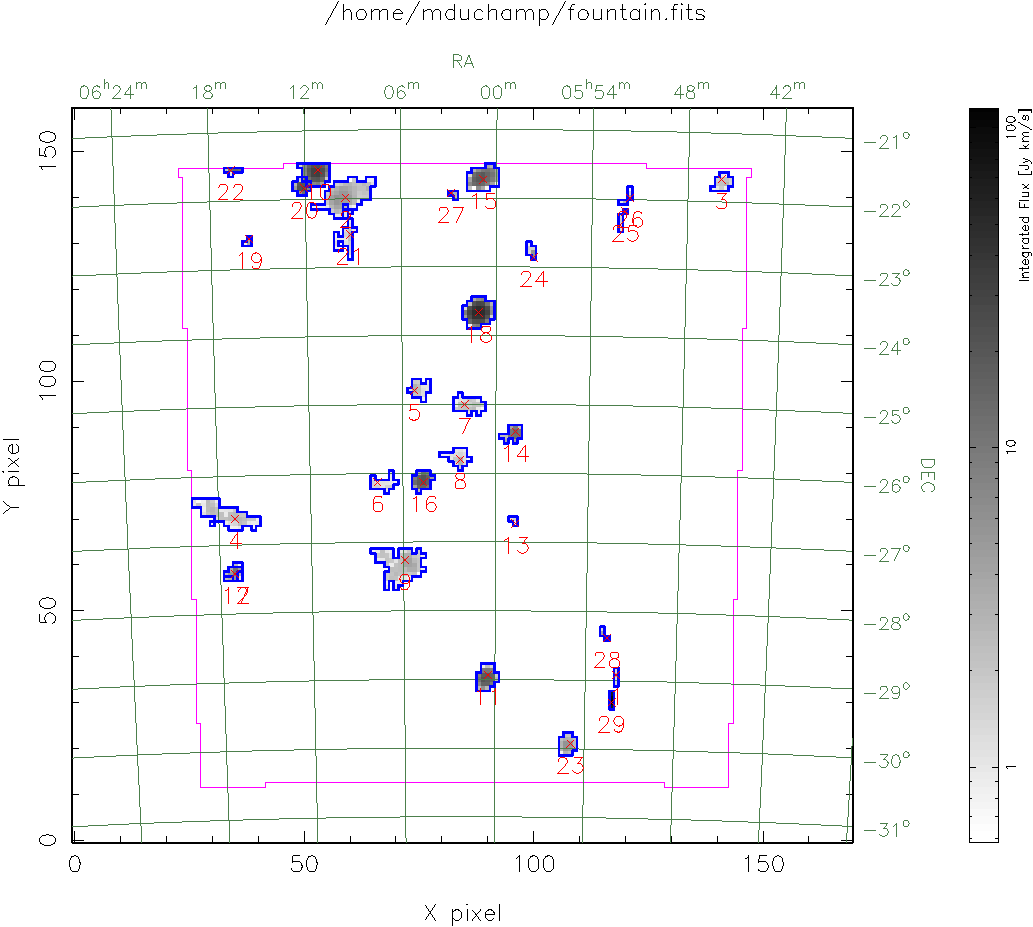
\includegraphics[width=\textwidth]{example_moment_map}
\end{center}
\caption{\footnotesize An example of the moment map created by
  \duchamp. The full extent of the cube is covered, and the 0th moment
  of each object is shown (integrated individually over all the
  detected channels). The purple line indicates the limit of the
  non-BLANK pixels.}
\label{fig-moment}
\end{figure}

Finally, a couple of images are optionally produced: a 0th moment map
of the cube, combining just the detected channels in each object,
showing the integrated flux in grey-scale; and a ``detection image'',
a grey-scale image where the pixel values are the number of channels
that spatial pixel is detected in. In both cases, if
\texttt{drawBorders = true}, a border is drawn around the spatial
extent of each detection, and if \texttt{drawBlankEdges = true}, the
purple line dividing BLANK and non-BLANK pixels (as described above)
is drawn. An example moment map is shown in Fig.~\ref{fig-moment}.
The production or otherwise of these images is governed by the
\texttt{flagMaps} parameter.

The moment map is also displayed in a PGPlot XWindow (with the
\texttt{/xs} display option). This feature can be turned off by
setting \texttt{flagXOutput = false} -- this might be useful if
running \duchamp on a terminal with no window display capability, or
if you have set up a script to run it in a batch mode.

The purpose of these images are to provide a visual guide to where the
detections have been made, and, particularly in the case of the moment
map, to provide an indication of the strength of the source. In both
cases, the detections are numbered (in the same sense as the output
list and as the spectral plots), and the spatial borders are marked
out as for the cutout images in the spectra file. Both these images
are saved as postscript files (given by the parameters
\texttt{momentMap} and \texttt{detectionMap} respectively), with the
latter also displayed in a \textsc{pgplot} window (regardless of the
state of \texttt{flagMaps}).
 %Outputs
\newpage
\newpage
\secA{Notes and hints on the use of \duchamp}
\label{sec-notes}

In using \duchamp, the user has to make a number of decisions about
the way the program runs. This section is designed to give the user
some idea about what to choose.

The main choice is whether to alter the cube to try and enhance the
detectability of objects, by either smoothing or reconstructing via
the \atrous method. The main benefits of both methods are the marked
reduction in the noise level, leading to regularly-shaped detections,
and good reliability for faint sources.

The main drawback with the \atrous method is the long execution time:
to reconstruct a $170\times160\times1024$ (\hipass) cube often
requires three iterations and takes about 20-25 minutes to run
completely. Note that this is for the more complete three-dimensional
reconstruction: using \texttt{reconDim=1} makes the reconstruction
quicker (the full program then takes less than 5 minutes), but it is
still the largest part of the time.

The smoothing procedure is computationally simpler, and thus quicker,
than the reconstruction. The spectral Hanning method adds only a very
small overhead on the execution, and the spatial Gaussian method,
while taking longer, will be done (for the above example) in less than
2 minutes. Note that these times will depend on the size of the
filter/kernel used: a larger filter means more calculations.

The searching part of the procedure is much quicker: searching an
un-reconstructed cube leads to execution times of less than a
minute. Alternatively, using the ability to read in previously-saved
reconstructed arrays makes running the reconstruction more than once a
more feasible prospect.

On the positive side, the shape of the detections in a cube that has
been reconstructed or smoothed will be much more regular and smooth --
the ragged edges that objects in the raw cube possess are smoothed by
the removal of most of the noise. This enables better determination of
the shapes and characteristics of objects.

A further point to consider when using the reconstruction is that if
the two-dimensional reconstruction is chosen (\texttt{reconDim=2}), it
can be susceptible to edge effects. If the valid area in the cube (\ie
the part that is not BLANK) has non-rectangular edges, the convolution
can produce artefacts in the reconstruction that mimic the edges and
can lead (depending on the selection threshold) to some spurious
sources. Caution is advised with such data -- the user is advised to
check carefully the reconstructed cube for the presence of such
artefacts. Note, however, that the 1- and 3-dimensional
reconstructions are \emph{not} susceptible in the same way, since the
spectral direction does not generally exhibit these BLANK edges, and
so we recommend the use of either of these.

If one chooses the reconstruction method, a further decision is
required on the signal-to-noise cutoff used in determining acceptable
wavelet coefficients. A larger value will remove more noise from the
cube, at the expense of losing fainter sources, while a smaller value
will include more noise, which may produce spurious detections, but
will be more sensitive to faint sources. Values of less than about
$3\sigma$ tend to not reduce the noise a great deal and can lead to
many spurious sources (this depends, of course on the cube itself).

The smoothing options have less parameters to consider: basically just
the size of the smoothing function or kernel. Spectrally smoothing
with a Hanning filter of width 3 (the smallest possible) is very
efficient at removing spurious one-channel objects that may result
just from statistical fluctuations of the noise. One may want to use
larger widths or kernels of larger size to look for features of a
particular scale in the cube.

When it comes to searching, the FDR method produces more reliable
results than simple sigma-clipping, particularly in the absence of
reconstruction.  However, it does not work in exactly the way one
would expect for a given value of \texttt{alpha}. For instance,
setting fairly liberal values of \texttt{alpha} (say, 0.1) will often
lead to a much smaller fraction of false detections (\ie much less
than 10\%). This is the effect of the merging algorithms, that combine
the sources after the detection stage, and reject detections not
meeting the minimum pixel or channel requirements.  It is thus better
to aim for larger \texttt{alpha} values than those derived from a
straight conversion of the desired false detection rate.

Finally, as \duchamp is still undergoing development, there are some
elements that are not fully developed. In particular, it is not as
clever as I would like at avoiding interference. The ability to place
requirements on the minimum number of channels and pixels partially
circumvents this problem, but work is being done to make \duchamp
smarter at rejecting signals that are clearly (to a human eye at
least) interference. See the following section for further
improvements that are planned.
 %Notes and hints on the use of \duchamp
\newpage
\secA{Future developments}

Here are lists of planned improvements and a wish-list of
features that would be nice to include (but are not planned in the
immediate future). Let me know if there are items not on these lists,
or items on the list you would like prioritised.

Planned developments:
\begin{itemize}
\item Parallelisation of the code, to improve speed particularly on
multi-core machines.

\item Better determination of the noise characteristics of
  spectral-line cubes, including understanding how the noise is
  generated and developing a model for it. 
  
\item Include more source analysis. Examples could be: shape
  information; measurements of HI mass; more variety of measurements
  of velocity width and profile. 

\item Improved ability to reject interference, possibly on the
  spectral shape of features.

\item Ability to separate (de-blend) distinct sources that have been
  merged.
\end{itemize}

Wish-list:
\begin{itemize}
\item Incorporation of Swinburne's S2PLOT
\footnote{\href{http://astronomy.swin.edu.au/s2plot/}
{http://astronomy.swin.edu.au/s2plot/}} code for improved
visualisation. 
\item Link to lists of possible counterparts (\eg via NED/SIMBAD/other
  VO tools?). 

\item On-line web service interface, so a user can upload a cube and
  get back a source-list.

\item Embed \duchamp in a GUI, to move away from the text-based
  interaction.
\end{itemize}

\secA{Why ``\duchamp''?}

Well, it's important for a program to have a name, and the initial
working title of \emph{cubefind} was somewhat uninspiring. I wanted to
avoid the classic astronomical approach of designing a cute acronym,
and since it is designed to work on cubes, I looked at naming it after
a cubist. \emph{Picasso}, sadly, was already taken \citep{minchin99},
so I settled on naming it after Marcel Duchamp, another cubist, but
also one of the first artists to work with ``found objects''.

 %Future developments
\newpage
% -----------------------------------------------------------------------
% acknowledgements.tex: Acknowledgements & thankyous
% -----------------------------------------------------------------------
% Copyright (C) 2006, Matthew Whiting, ATNF
%
% This program is free software; you can redistribute it and/or modify it
% under the terms of the GNU General Public License as published by the
% Free Software Foundation; either version 2 of the License, or (at your
% option) any later version.
%
% Duchamp is distributed in the hope that it will be useful, but WITHOUT
% ANY WARRANTY; without even the implied warranty of MERCHANTABILITY or
% FITNESS FOR A PARTICULAR PURPOSE.  See the GNU General Public License
% for more details.
%
% You should have received a copy of the GNU General Public License
% along with Duchamp; if not, write to the Free Software Foundation,
% Inc., 59 Temple Place, Suite 330, Boston, MA 02111-1307, USA
%
% Correspondence concerning Duchamp may be directed to:
%    Internet email: Matthew.Whiting [at] atnf.csiro.au
%    Postal address: Dr. Matthew Whiting
%                    Australia Telescope National Facility, CSIRO
%                    PO Box 76
%                    Epping NSW 1710
%                    AUSTRALIA
% -----------------------------------------------------------------------
\secA{Acknowledgements}

Thanks are due to the many people who have provided assistance and
advice during the development and testing of \duchamp, particularly
Ivy Wong, Kathrin Wolfinger, Tobias Westmeier, Sara Shakouri, Mary
Putman, Cormac Purcell, Attila Popping, Tara Murphy, Enno Middelberg,
Korinne McDonnell, Malte Marquarding, Philip Lah, Russell Jurek, Simon
Guest, Jose Francisco Gomez, BiQing For, Luca Cortese, Mark
Calabretta, David Barnes and Robbie Auld. Additionally, Emil Lenc and
Anita Richards both provided valuable comments on the journal paper
that have helped the descriptions therein. I'd like to thank the
members of the ASKAP Working Group 2 (Source Finding) for their
interest and feedback - \duchamp has been considered as part of the
development of ASKAP Survey Science Projects, and this has driven
further development of the core \duchamp software.

The graphics in \duchamp are created using the
\textsc{pgplot}\footnote{http://www.astro.caltech.edu/$\sim$tjp/pgplot/}
library, FITS file access is controlled through the
\textsc{cfitsio}\footnote{http://heasarc.gsfc.nasa.gov/docs/software/fitsio/fitsio.html}
library \citep{pence99}, while the world-coordinate transformations
are performed using the
\textsc{wcslib}\footnote{http://www.atnf.csiro.au/people/mcalabre/WCS/index.html}
library (described in \citet{calabretta02}).

The bulk of this work was conducted as part of a CSIRO Emerging
Science Postdoctoral Fellowship, and \duchamp continues to be
maintained both as a standalone package and as part of the software
development effort for the ASKAP telescope. This work was supported by
the NCI National Facility at the ANU.



%%% Local Variables: 
%%% mode: latex
%%% TeX-master: "Guide"
%%% End: 
 %Acknowledgements

\newpage
\ifPDF
\pdfbookmark[1]{References}{references}
\fi
%\bibliographystyle{plainnat}
%%\bibliographystyle{hapj}
%%\bibliographystyle{plainnaturl}
%%\bibliographystyle{mn2e}
%%\bibliography{mnemonic,MasterBibliography}
%\bibliography{guide}
%%\bibliography{Guide-new}

%\newpage
%\ifPDF
%\pdfbookmark[1]{References}{references}
%\fi
%\ifPDF
\begin{thebibliography}{12}
\expandafter\ifx\csname natexlab\endcsname\relax\def\natexlab#1{#1}\fi
\expandafter\ifx\csname url\endcsname\relax
  \def\url#1{{\tt #1}}\fi

\bibitem[{Calabretta} and {Greisen}(2002)]{calabretta02}
M.R. {Calabretta} and E.W. {Greisen}.
\newblock {``Representations of celestial coordinates in FITS''}.
\newblock
\href{http://adsabs.harvard.edu/cgi-bin/nph-bib_query?bibcode=2002A%26A...395%.1077C&db_key=AST}%
{{\em A\&A}, 395:\penalty0 1077--1122, December 2002.}
%\newblock URL
.

\bibitem[{Greisen} and {Calabretta}(2002)]{greisen02}
E.W. {Greisen} and M.R. {Calabretta}.
\newblock {``Representations of world coordinates in FITS''}.
\newblock
\href{http://adsabs.harvard.edu/cgi-bin/nph-bib_query?bibcode=2002A%26A...395%.1061G&db_key=AST}%
{{\em A\&A}, 395:\penalty0 1061--1075, December 2002.}
%\newblock URL
%  \url{.

\bibitem[{Greisen} et~al.(2006){Greisen}, {Calabretta}, Valdes, and
  Allen]{greisen06}
E.W. {Greisen}, M.R. {Calabretta}, F.G. Valdes, and S.L. Allen.
\newblock {Representations of spectral coordinates in FITS}.
\newblock 
\href{http://adsabs.harvard.edu/abs/2006A%26A...446..747G}{\emph{A\&A}, 446:\penalty0 747--771, 2006.}

\bibitem[{Hanisch} et~al.(2001){Hanisch}, {Farris}, {Greisen}, {Pence},
  {Schlesinger}, {Teuben}, {Thompson}, and {Warnock}]{hanisch01}
R.J. {Hanisch}, A.~{Farris}, E.W. {Greisen}, W.D. {Pence}, B.M. {Schlesinger},
  P.J. {Teuben}, R.W. {Thompson}, and A.~{Warnock}.
\newblock {``Definition of the Flexible Image Transport System (FITS)''}.
\newblock 
\href{http://adsabs.harvard.edu/cgi-bin/nph-bib_query?bibcode=2001A%26A...376%
..359H&db_key=AST}%
{{\em A\&A}, 376:\penalty0 359--380, September 2001.}
%\newblock URL
%  \url.

\bibitem[{Hopkins} et~al.(2002){Hopkins}, {Miller}, {Connolly}, {Genovese},
  {Nichol}, and {Wasserman}]{hopkins02}
A.M. {Hopkins}, C.J. {Miller}, A.J. {Connolly}, C.~{Genovese}, R.C. {Nichol},
  and L.~{Wasserman}.
\newblock {``A New Source Detection Algorithm Using the False-Discovery
  Rate''}.
\newblock 
\href{http://adsabs.harvard.edu/cgi-bin/nph-bib_query?bibcode=2002AJ....123.1%
086H&db_key=AST}%
{{\em AJ}, 123:\penalty0 1086--1094, February 2002.}
%\newblock URL
%  \url.

\bibitem[Lutz(1980)]{lutz80}
R.K. Lutz.
\newblock {``An algorithm for the real time analysis of digitised images''}.
\newblock {\em The Computer Journal}, 23:\penalty0 262--269, 1980.

\bibitem[{Meyer} et~al.(2004)]{meyer04-alt}
M.J. {Meyer} et~al.
\newblock {``The HIPASS catalogue - {\sc I}. Data presentation''}.
%\newblock 
\href{http://adsabs.harvard.edu/cgi-bin/nph-bib_query?bibcode=2004MNRAS.350.1%
195M&db_key=AST}%
{{\em MNRAS}, 350:\penalty0 1195--1209, June 2004.}
%\newblock URL
%  \url.

\bibitem[{Miller} et~al.(2001){Miller}, {Genovese}, {Nichol}, {Wasserman},
  {Connolly}, {Reichart}, {Hopkins}, {Schneider}, and {Moore}]{miller01}
C.J. {Miller}, C.~{Genovese}, R.C. {Nichol}, L.~{Wasserman}, A.~{Connolly},
  D.~{Reichart}, A.~{Hopkins}, J.~{Schneider}, and A.~{Moore}.
\newblock {``Controlling the False-Discovery Rate in Astrophysical Data
  Analysis''}.
\newblock 
\href{http://adsabs.harvard.edu/cgi-bin/nph-bib_query?bibcode=2001AJ....122.3%
492M&db_key=AST}%
{{\em AJ}, 122:\penalty0 3492--3505, December 2001.}
%\newblock URL
%  \url.

\bibitem[Minchin(1999)]{minchin99}
R.F. Minchin.
\newblock {``Finding the Bivariate Brightness Distribution of Galaxies from an
  HI Selected Sample''}.
\newblock \href{http://adsabs.harvard.edu/abs/1999PASA...16...12M}{{\em PASA}, 16:\penalty0 12--17, 1999.}

\bibitem[{Pence}(1999)]{pence99}
W.~{Pence}.
\newblock {CFITSIO, v2.0: A New Full-Featured Data Interface}.
\newblock \href{http://adass.org/adass/proceedings/adass98/pencewd/}%
{In {D.~M.~Mehringer, R.~L.~Plante, \& D.~A.~Roberts}, editor,
  \emph{Astronomical Data Analysis Software and Systems VIII}, volume 172 of
  \emph{Astronomical Society of the Pacific Conference Series}, page 487, 1999.}

\bibitem[Starck and Murtagh(2002)]{starck02a}
J.-L. Starck and F.~Murtagh.
\newblock {\em {``Astronomical Image and Data Analysis''}}.
\newblock Springer, 2002.

\bibitem[Whiting(2012)]{whiting12}
M.~T. Whiting.
\newblock {\textsc{duchamp}: a 3D source finder for spectral-line data}.
\newblock \href{http://onlinelibrary.wiley.com/doi/10.1111/j.1365-2966.2012.20548.x/full}%
{\emph{MNRAS}, 421:\penalty0 3242--3256, 2012.}

\end{thebibliography}

%\else
%\begin{thebibliography}{}

\bibitem[\protect\citeauthoryear{{Calabretta} \& {Greisen}}{{Calabretta} \&
  {Greisen}}{2002}]{calabretta02}
{Calabretta} M.,  {Greisen} E.,  2002, A\&A, 395, 1077

\bibitem[\protect\citeauthoryear{{Greisen} \& {Calabretta}}{{Greisen} \&
  {Calabretta}}{2002}]{greisen02}
{Greisen} E.,  {Calabretta} M.,  2002, A\&A, 395, 1061

\bibitem[\protect\citeauthoryear{{Hanisch}, {Farris}, {Greisen}, {Pence},
  {Schlesinger}, {Teuben}, {Thompson} \& {Warnock}}{{Hanisch}
  et~al.}{2001}]{hanisch01}
{Hanisch} R.,  {Farris} A.,  {Greisen} E.,  {Pence} W.,  {Schlesinger} B.,
  {Teuben} P.,  {Thompson} R.,    {Warnock} A.,  2001, A\&A, 376, 359

\bibitem[\protect\citeauthoryear{{Hopkins}, {Miller}, {Connolly}, {Genovese},
  {Nichol} \& {Wasserman}}{{Hopkins} et~al.}{2002}]{hopkins02}
{Hopkins} A.,  {Miller} C.,  {Connolly} A.,  {Genovese} C.,  {Nichol} R.,
  {Wasserman} L.,  2002, AJ, 123, 1086

\bibitem[\protect\citeauthoryear{Lutz}{Lutz}{1980}]{lutz80}
Lutz R.,  1980, The Computer Journal, 23, 262

\bibitem[\protect\citeauthoryear{{Meyer} et~al.,}{{Meyer}
  et~al.}{2004}]{meyer04:trunc}
{Meyer} M.,  et~al., 2004, MNRAS, 350, 1195

\bibitem[\protect\citeauthoryear{{Miller}, {Genovese}, {Nichol}, {Wasserman},
  {Connolly}, {Reichart}, {Hopkins}, {Schneider} \& {Moore}}{{Miller}
  et~al.}{2001}]{miller01}
{Miller} C.,  {Genovese} C.,  {Nichol} R.,  {Wasserman} L.,  {Connolly} A.,
  {Reichart} D.,  {Hopkins} A.,  {Schneider} J.,    {Moore} A.,  2001, AJ, 122,
  3492

\bibitem[\protect\citeauthoryear{Minchin}{Minchin}{1999}]{minchin99}
Minchin R.,  1999, PASA, 16, 12

\bibitem[\protect\citeauthoryear{Starck \& Murtagh}{Starck \&
  Murtagh}{2002}]{starck02:book}
Starck J.-L.,  Murtagh F.,  2002, {``Astronomical Image and Data Analysis''}.
Springer

\end{thebibliography}

%\fi

\appendix
\newpage
\secA{Obtaining and installing \duchamp}
\label{app-install}

\secB{Installing}
The \duchamp web page can be found at the following location:\\
\href{http://www.atnf.csiro.au/people/Matthew.Whiting/Duchamp}%
{http://www.atnf.csiro.au/people/Matthew.Whiting/Duchamp}\\
Here you can find a gzipped tar archive of the source code that can be
downloaded and extracted, as well as this User's Guide in postscript
and hyperlinked PDF formats.

To build \duchamp, you will need three main external libraries:
\textsc{pgplot}, \textsc{cfitsio} (this needs to be version 2.5 or
greater -- version 3+ is better) and \textsc{wcslib}. If these are not
present on your system, you can download them from the following
locations:
\begin{itemize}
\item \textsc{pgplot}:
\href{http://www.astro.caltech.edu/~tjp/pgplot/}%
{\footnotesize http://www.astro.caltech.edu/~tjp/pgplot/}
\item \textsc{cfitsio}:
\href{http://heasarc.gsfc.nasa.gov/docs/software/fitsio/fitsio.html}%
{\footnotesize http://heasarc.gsfc.nasa.gov/docs/software/fitsio/fitsio.html}
\item \textsc{wcslib}:
\href{http://www.atnf.csiro.au/people/Mark.Calabretta/WCS/index.html}%
{\footnotesize http://www.atnf.csiro.au/people/Mark.Calabretta/WCS/index.html}
\end{itemize}

\duchamp can be built on Unix/Linux systems by typing (assuming that
the prompt your terminal provides is a \texttt{> } -- don't type this
character!):
\begin{quote}
{\footnotesize
\texttt{%
> ./configure\\
> make\\
> make clean (optional -- to remove the object files)}
}
\end{quote}

Run in this manner, \texttt{configure} should find all the necessary
libraries, but if some libraries have been installed in non-standard
locations, it may fail. In this case, you can specify additional
directories to look in by giving extra command-line arguments. There
are separate options for library files (eg. libcpgplot.a) and header
files (eg. cpgplot.h).

For example, suppose \textsc{wcslib} had been locally installed in the
directory \texttt{/home/mduchamp/wcslib}. There will then be two
libraries created that are likely to be in the following
subdirectories: \texttt{C/} and \texttt{pgsbox/}. Each subdirectory
needs to be searched for library and header files, so one could build
Duchamp by typing:
\begin{quote}
{\footnotesize
\texttt{%
>  ./configure $\backslash$ \\ 
LIBDIRS="/home/mduchamp/wcslib/C /home/mduchamp/wcslib/pgsbox" 
$\backslash$\\
INCDIRS="/home/mduchamp/wcslib/C /home/mduchamp/wcslib/pgsbox"}
}
\end{quote}
And then just run make in the usual fashion:
\begin{quote}
{\footnotesize
\texttt{> make}
}
\end{quote}

This will produce the executable \texttt{Duchamp}. You can verify that
it is running correctly by running the verification shell script:
\begin{quote}
{\footnotesize
\texttt{> VerifyDuchamp.sh}
}
\end{quote}
This will use a dummy FITS image in the \texttt{verification/}
directory -- this image has some Gaussian random noise, with five
Gaussian sources present, plus a dummy WCS. The script runs
Duchamp on this image with three different sets of inputs, and
compares to known results, looking for differences and reporting
any. There should be none reported if everything is working correctly.

\secB{Running \duchamp}
You can then run \duchamp on your own data. This can be done in one
of two ways. The first is:
\begin{quote}
{\footnotesize
\texttt{> Duchamp -f [FITS file]}
}
\end{quote}
where \texttt{[FITS file]} is the file you wish to search. This method
simply uses the default values of all parameters.

The second method allows some determination of the parameter values by
the user. Type:
\begin{quote}
{\footnotesize
\texttt{> Duchamp -p [parameter file]}
}
\end{quote}
where \texttt{[parameterFile]} is a file with the input parameters,
including the name of the cube you want to search. There are two
example input files included with the distribution. The smaller one,
\texttt{InputExample}, shows the typical parameters one might want to
set. The large one, \texttt{InputComplete}, lists all possible
parameters that can be entered, and a brief description of them. To
get going quickly, just replace the \texttt{"your-file-here"} in the
\texttt{InputExample} file with your image name, and type
\begin{quote}
{\footnotesize
\texttt{> Duchamp -p InputExample}
}
\end{quote}

The following appendices provide details on the individual parameters,
and show examples of the output files that \duchamp produces.

\secB{Feedback}
It may happen that you discover bugs or problems with \duchamp, or you
have suggestions for improvements or additional features to be
included in future releases. You can submit a ``ticket'' (a trackable
bug report) at the \duchamp Trac wiki at the following location:\\
\href{http://sourcecode.atnf.csiro.au/cgi-bin/trac\_duchamp.cgi/newticket}%
{\footnotesize 
http://sourcecode.atnf.csiro.au/cgi-bin/trac\_duchamp.cgi/newticket}
\\(there is a link to this page from the Duchamp website).

There is also an email exploder, duchamp-user\textbf{[at]}atnf.csiro.au,
that users can subscribe to keep up to date with changes, updates, and
other news about \duchamp. To subscribe, send an email (from the
account you wish to subscribe to the list) to
duchamp-user-request\textbf{[at]}atnf.csiro.au with the single word
``subscribe'' in the body of the message. To be removed from this
list, send a message with ``unsubscribe'' in its body to the same
address.

 %Obtaining and installing \duchamp
\newpage
\secA{Available parameters}
\label{app-param}

The full list of parameters that can be listed in the input file are
given here. If not listed, they take the default value given in
parentheses. Since the order of the parameters in the input file does
not matter, they are grouped here in logical sections.

\secB*{Input related}
\begin{entry}
\item[ImageFile (no default assumed)] The filename of the
  data cube to be analysed.
\item[flagSubsection \texttt{[false]}] A flag to indicate whether one
  wants a subsection of the requested image.
\item[Subsection \texttt{[ [*,*,*] ]}] The requested subsection, which
  should be specified in the format \texttt{[x1:x2,y1:y2,z1:z2]},
  where the limits are inclusive. If the full range of a dimension is
  required, use a \texttt{*}, \eg if you want the full spectral range
  of a subsection of the image, use \texttt{[30:140,30:140,*]} (thus
  the default is the full cube).
\item[flagReconExists \texttt{[false]}] A flag to indicate whether the
  reconstructed array has been saved by a previous run of \duchamp. If
  set true, the reconstructed array will be read from the file given
  by \texttt{reconFile}, rather than calculated directly.
\item[reconFile (no default assumed)] The FITS file that contains the
  reconstructed array. If \texttt{flagReconExists} is true and this
  parameter is not defined, the default file searched will be
  determined by the \atrous\ parameters (see \S\ref{sec-recon}).
\item[flagSmoothExists \texttt{[false]}] A flag to indicate whether the
  Hanning-smoothed array has been saved by a previous run of \duchamp. If
  set true, the smoothed array will be read from the file given
  by \texttt{smoothFile}, rather than calculated directly.
\item[smoothFile (no default assumed)] The FITS file that contains the
  Hanning-smoothed array. If \texttt{flagSmoothExists} is true and
  this parameter is not defined, the default file searched will be
  determined by the Hanning width parameter (see
  \S\ref{sec-smoothing}).
\end{entry}

\secB*{Output related}
\begin{entry}
\item[OutFile \texttt{[duchamp-Results.txt]}] The file containing the
  final list of detections. This also records the list of input
  parameters.
\item[SpectraFile \texttt{[duchamp-Spectra.ps]}] The postscript file
  containing the resulting integrated spectra and images of the
  detections. 
\item[flagLog \texttt{[true]}] A flag to indicate whether intermediate
  detections should be logged.
\item[LogFile \texttt{[duchamp-Logfile.txt]}] The file in which
  intermediate detections are logged. These are detections that have
  not been merged. This is primarily for use in debugging and
  diagnostic purposes -- normal use of the program will probably not
  require this.
\item[flagOutputRecon \texttt{[false]}] A flag to say whether or not
  to save the reconstructed cube as a FITS file. The filename will be
  derived according to the naming scheme detailed in
  Section~\ref{sec-reconIO}.
\item[flagOutputResid \texttt{[false]}] As for
  \texttt{flagOutputRecon}, but for the residual array -- the
  difference between the original cube and the reconstructed cube. The
  filename will be derived according to the naming scheme detailed in
  Section~\ref{sec-reconIO}.
\item[flagOutputSmooth \texttt{[false]}] A flag to say whether or not
  to save the smoothed cube as a FITS file. The filename will be
  derived according to the naming scheme detailed in
  Section~\ref{sec-smoothing}.
\item[flagVOT \texttt{[false]}] A flag to say whether to create a
  VOTable file corresponding to the information in
  \texttt{outfile}. This will be an XML file in the Virtual
  Observatory VOTable format.
\item[votFile \texttt{[duchamp-Results.xml]}] The VOTable file with
  the list of final detections. Some input parameters are also
  recorded.
\item[flagKarma \texttt{[false]}] A flag to say whether to create a
  Karma annotation file corresponding to the information in
  \texttt{outfile}. This can be used as an overlay for the Karma
  programs such as \texttt{kvis}.
\item[karmaFile \texttt{[duchamp-Results.ann]}] The Karma annotation
  file showing the list of final detections. 
\item[flagMaps \texttt{[true]}] A flag to say whether to save
  postscript files showing the 0th moment map of the whole cube
  (parameter \texttt{momentMap}) and the detection image
  (\texttt{detectionMap}).
\item[momentMap \texttt{[duchamp-MomentMap.ps]}] A postscript file
  containing a map of the 0th moment of the detected sources, as well
  as pixel and WCS coordinates.
\item[detectionMap \texttt{[duchamp-DetectionMap.ps]}] A postscript
  file showing each of the detected objects, coloured in greyscale by
  the number of channels spanned by each pixel. Also shows pixel and
  WCS coordinates.
\item[flagXOutput \texttt{[true]}] A flag to say whether to display a
  0th moment map in a PGPlot Xwindow. This will be in addition to any
  that are saved to a file.
\end{entry}

\secB*{Modifying the cube}
\begin{entry}
\item[flagBlankPix \texttt{[true]}] A flag to say whether to remove
  BLANK pixels from the analysis -- these are pixels set to some
  particular value because they fall outside the imaged area.
\item[blankPixValue \texttt{[-8.00061]}] The value of the BLANK
  pixels, if this information is not contained in the FITS header (the
  usual procedure is to obtain this value from the header information
  -- in which case the value set by this parameter is ignored).
\item[flagMW \texttt{[false]}] A flag to say whether to ignore
  channels contaminated by Milky Way (or other) emission -- the
  searching algorithms will not look at these channels.
\item[maxMW \texttt{[112]}] The maximum channel number containing
  ``Milky Way'' emission.
\item[minMW \texttt{[75]}] The minimum channel number containing
  ``Milky Way'' emission. Note that the range specified by
  \texttt{maxMW} and \texttt{minMW} is inclusive.
\item[flagBaseline \texttt{[false]}] A flag to say whether to remove
  the baseline from each spectrum in the cube for the purposes of
  reconstruction and detection.
\end{entry}

\secB*{Detection related}

\secC*{General detection}
\begin{entry}
\item[flagNegative \texttt{[false]}] A flag to indicate that the
  features being searched for are negative. The cube will be inverted
  prior to searching.
\item[snrCut \texttt{[3.]}] The cut-off value for thresholding, in
  terms of number of $\sigma$ above the mean.
\item[threshold (no default assumed)] The actual value of the
  threshold. Normally the threshold is calculated from the cube's
  statistics, but the user can manually specify a value to be used
  that overrides the calculated value. If this is not specified, the
  calculated value is used. Also, when the FDR method is requested
  (see below), the value of the \texttt{threshold} parameter is
  ignored. 
\item[flagGrowth \texttt{[false]}] A flag indicating whether or not to
  grow the detected objects to a smaller threshold.
\item[growthCut \texttt{[2.]}] The smaller threshold using in growing
  detections. In units of $\sigma$ above the mean.
\item[beamSize \texttt{[10.]}] The size of the beam in pixels. If the
  header keywords BMAJ and BMIN are present, then these will be used
  to calculate the beam size, and this parameter will be ignored. 
\end{entry}

\secC*{\Atrous\ reconstruction}
\begin{entry}
\item [flagATrous \texttt{[true]}] A flag indicating whether or not to
  reconstruct the cube using the \atrous\ wavelet
  reconstruction. See \S\ref{sec-recon} for details.
\item[reconDim \texttt{[3]}] The number of dimensions to use in the
  reconstruction. 1 means reconstruct each spectrum separately, 2
  means each channel map is done separately, and 3 means do the whole
  cube in one go.
\item[scaleMin \texttt{[1]}] The minimum wavelet scale to be used in the
  reconstruction. A value of 1 means ``use all scales''.
\item[snrRecon \texttt{[4]}] The thresholding cutoff used in the
  reconstruction -- only wavelet coefficients this many $\sigma$ above
  the mean (or greater) are included in the reconstruction. 
\item[filterCode \texttt{[1]}] The code number of the filter to use in
  the reconstruction. The options are:
  \begin{itemize}
  \item \textbf{1:} B$_3$-spline filter: coefficients = 
    $(\frac{1}{16}, \frac{1}{4}, \frac{3}{8}, \frac{1}{4}, \frac{1}{16})$
  \item \textbf{2:} Triangle filter: coefficients = 
    $(\frac{1}{4}, \frac{1}{2}, \frac{1}{4})$
  \item \textbf{3:} Haar wavelet: coefficients = 
    $(0, \frac{1}{2}, \frac{1}{2})$
  \end{itemize}
\end{entry}

\secC*{Smoothing the cube}
\begin{entry}
\item [flagSmooth \texttt{[false]}] A flag indicating whether to
  Hanning-smooth the cube. See \S\ref{sec-smoothing} for details.
\item [hanningWidth \texttt{[5]}] The width of the Hanning smoothing
kernel. 
\end{entry}

\secC*{FDR method}
\begin{entry}
\item[flagFDR \texttt{[false]}] A flag indicating whether or not to use
  the False Discovery Rate method in thresholding the pixels.
\item[alphaFDR \texttt{[0.01]}] The $\alpha$ parameter used in the FDR
analysis. The average number of false detections, as a fraction of the
total number, will be less than $\alpha$ (see \S\ref{sec-detection}).
\end{entry}

\secC*{Merging detections}
\begin{entry}
\item[minPix \texttt{[2]}] The minimum number of spatial pixels for a
  single detection to be counted.
\item[minChannels \texttt{[3]}] The minimum number of consecutive
  channels that must be present in a detection.
\item[flagAdjacent \texttt{[true]}] A flag indicating whether to use
  the ``adjacent pixel'' criterion to decide whether to merge
  objects. If not, the next two parameters are used to determine
  whether objects are within the necessary thresholds.
\item[threshSpatial \texttt{[3.]}] The maximum allowed minimum spatial
  separation (in pixels) between two detections for them to be merged
  into one. Only used if \texttt{flagAdjacent = false}.
\item[threshVelocity \texttt{[7.]}] The maximum allowed minimum channel
  separation between two detections for them to be merged into
  one. 
\end{entry}

\secC*{Other parameters}
\begin{entry}
\item[spectralMethod \texttt{[peak]}] This indicates which method is used
  to plot the output spectra: \texttt{peak} means plot the spectrum
  containing the detection's peak pixel; \texttt{sum} means sum the
  spectra of each detected spatial pixel, and correct for the beam
  size. Any other choice defaults to \texttt{peak}.
\item[spectralUnits \texttt{[km/s]}] The user can specify the units of
  the spectral axis. Assuming the WCS of the FITS file is valid, the
  spectral axis is transformed into velocity, and put into these units
  for all output and for calculations such as the integrated flux of a
  detection.
\item[drawBorders \texttt{[true]}] A flag indicating whether borders
  are to be drawn around the detected objects in the moment maps
  included in the output (see for example Fig.~\ref{fig-spect}).
\item[drawBlankEdges \texttt{[true]}] A flag indicating whether to
 draw the dividing line between BLANK and non-BLANK pixels on the
 2-dimensional images (see for example Fig.~\ref{fig-moment}).
\item[verbose \texttt{[true]}] A flag indicating whether to print the
  progress of computationally-intensive algorithms (such as the
  searching and merging) to screen.
\end{entry}

 %Available parameters
\newpage
\secA{Example parameter files}
\label{app-input}

This is what a typical parameter file would look like.

\begin{verbatim}
imageFile       /home/mduchamp/fountain.fits
logFile         logfile.txt
outFile         results.txt
spectraFile     spectra.ps
flagSubsection  false
flagOutputRecon false
flagOutputResid 0
flagBlankPix    1
flagMW          1
minMW           75
maxMW           112
minPix          3
flagGrowth      1
growthCut       1.5
flagATrous      0
scaleMin        1
snrRecon        4
flagFDR         1
alphaFDR        0.1
numPixPSF       20
snrCut          3
threshSpatial   3
threshVelocity  7
\end{verbatim}

Note that, as in this example, the flag parameters can be entered as
strings (true/false) or integers (1/0). Also, note that it is not
necessary to include all these parameters in the file, only those that
need to be changed from the defaults (as listed in
Appendix~\ref{app-param}), which in this case would be very few. A
minimal parameter file might look like:
\begin{verbatim}
imageFile       /home/mduchamp/fountain.fits
flagLog         false
flagATrous      1
snrRecon        3
snrCut          2.5
minChannels     4
\end{verbatim}
This will reconstruct the cube with a lower SNR value than the
default, select objects at a lower threshold,  with a looser minimum
channel requirement, and not keep a log of the intermediate
detections. 

The following page demonstrates how the parameters are presented to
the user, both on the screen at execution time, and in the output and
log files. On each line, there is a description on the parameter, the
relevant parameter name that is used in the input file (if there is
one that the user can enter), and the value of the parameter being
used.

%\begin{sideways}
%Typical presentation of parameters in output and log files:  
%\begin{minipage}{170mm}
{\scriptsize
\begin{verbatim}
---- Parameters ----
Image to be analysed.........................[imageFile]  =  /path/fountain.fits
Intermediate Logfile...........................[logFile]  =  duchamp-Logfile.txt
Final Results file.............................[outFile]  =  duchamp-Results.txt
Spectrum file..............................[spectraFile]  =  duchamp-Spectra.ps	  
0th Moment Map...............................[momentMap]  =  duchamp-MomentMap.ps
Detection Map.............................[detectionMap]  =  duchamp-DetectionMap.ps
Saving reconstructed cube?.............[flagoutputrecon]  =  false
Saving residuals from reconstruction?..[flagoutputresid]  =  false
------
Searching for Negative features?..........[flagNegative]  =  false
Fixing Blank Pixels?......................[flagBlankPix]  =  true
Blank Pixel Value.......................................  =  -8.00061
Removing Milky Way channels?....................[flagMW]  =  true
Milky Way Channels.......................[minMW - maxMW]  =  75-112
Beam Size (pixels)......................................  =  10.1788
Removing baselines before search?.........[flagBaseline]  =  false
Minimum # Pixels in a detection.................[minPix]  =  2
Minimum # Channels in a detection..........[minChannels]  =  3
Growing objects after detection?............[flagGrowth]  =  false
Using A Trous reconstruction?...............[flagATrous]  =  true
Number of dimensions in reconstruction........[reconDim]  =  3
Minimum scale in reconstruction...............[scaleMin]  =  1
SNR Threshold within reconstruction...........[snrRecon]  =  4
Filter being used for reconstruction........[filterCode]  =  1 (B3 spline function)
Using FDR analysis?............................[flagFDR]  =  false
SNR Threshold...................................[snrCut]  =  3
Using Adjacent-pixel criterion?...........[flagAdjacent]  =  true
Max. velocity separation for merging....[threshVelocity]  =  7
Method of spectral plotting.............[spectralMethod]  =  peak
\end{verbatim}
}
%\end{minipage}
%\end{sideways}
 %Example parameter files
\newpage
\secA{Example results file}
\label{app-output}
This the typical content of an output file, after running \duchamp\
with the parameters illustrated on the previous page. 

{\scriptsize 
  \begin{verbatim}
Results of the \duchamp\ source finder: Tue May 23 14:51:38 2006
---- Parameters ----
      (... omitted for clarity -- see previous page for examples...)
--------------------
Total number of detections = 25
--------------------
------------------------------------------------------------------------------------------------------------------------------------------------------
 Obj#       Name     X     Y     Z           RA          DEC      VEL     w_RA    w_DEC   w_VEL     F_int    F_peak  X1  X2  Y1  Y2  Z1  Z2  Npix Flag
                                                               [km/s] [arcmin] [arcmin]  [km/s] [Jy km/s] [Jy/beam]                         [pix]     
------------------------------------------------------------------------------------------------------------------------------------------------------
    1 J0618-2532  30.2  86.0 113.3  06:18:12.54 -25:32:44.79  208.502    45.17    34.61  26.383    24.394     0.350  25  35  82  90 112 114   137    E
    2 J0609-2156  59.5 140.6 114.6  06:09:19.66 -21:56:31.20  225.572    44.39    31.47  65.957    16.128     0.213  55  65 137 144 113 118   153     
    3 J0545-2143 141.2 143.2 114.8  05:45:51.71 -21:43:36.20  228.470    19.61    16.66  26.383     2.412     0.090 139 143 142 145 114 116    29     
    4 J0617-2633  33.3  70.8 115.6  06:17:25.52 -26:33:33.83  238.736    65.02    30.10  26.383     9.776     0.117  26  41  68  75 115 117   104    E
    5 J0601-2500  86.2  94.9 117.9  06:01:39.54 -25:00:32.46  269.419    27.99    24.02  26.383     3.920     0.124  83  89  92  97 117 119    44     
    6 J0602-2547  84.0  83.1 118.0  06:02:18.29 -25:47:31.69  270.319    20.01    19.99  26.383     2.999     0.118  82  86  81  85 117 119    34     
    7 J0547-2448 133.0  97.2 118.7  05:47:52.53 -24:48:38.16  279.113    19.72    12.54  26.383     1.474     0.074 131 135  96  98 118 120    21     
    8 J0606-2719  71.1  60.0 121.3  06:06:10.99 -27:19:48.61  314.090    52.36    39.59  39.574    14.268     0.150  65  77  55  64 120 123   154     
    9 J0611-2137  52.4 145.3 162.5  06:11:20.92 -21:37:29.57  857.955    32.39    23.49 118.722    43.178     0.410  49  56 142 147 158 167   265    E
   10 J0600-2859  89.7  35.3 202.4  06:00:34.08 -28:59:00.43 1383.160    23.93    24.10 171.487    24.439     0.173  87  92  33  38 196 209   271     
   11 J0558-2638  95.4  70.3 223.1  05:58:53.03 -26:38:45.91 1656.140    11.93    12.07  92.339     1.045     0.063  94  96  69  71 220 227    18     
   12 J0617-2723  34.7  58.3 227.4  06:17:07.07 -27:23:50.65 1712.868    16.75    23.53 290.209     8.529     0.093  33  36  56  61 215 237   118     
   13 J0558-2525  95.8  88.6 231.7  05:58:49.27 -25:25:33.60 1770.134    27.87    24.16 237.444    12.863     0.115  92  98  86  91 221 239   175     
   14 J0600-2141  88.8 144.4 232.5  06:00:54.02 -21:41:57.06 1780.188    27.96    24.13 224.252    30.743     0.166  86  92 142 147 222 239   344    E
   15 J0615-2634  40.0  70.8 232.6  06:15:25.50 -26:34:20.04 1782.214    12.44    15.69  52.765     2.084     0.068  39  41  69  72 231 235    31     
   16 J0604-2606  76.0  78.4 233.0  06:04:41.13 -26:06:21.19 1787.226    24.13    23.87 211.061    23.563     0.155  73  78  76  81 225 241   278     
   17 J0601-2340  87.9 114.9 235.8  06:01:08.83 -23:40:19.37 1824.122    31.95    28.09 237.444    82.380     0.297  85  92 112 118 227 245   647     
   18 J0615-2235  38.2 130.5 254.5  06:15:32.09 -22:35:37.24 2070.934    12.29    11.70 105.531     1.555     0.070  37  39 129 131 249 257    24     
   19 J0617-2305  31.4 122.8 258.1  06:17:33.45 -23:05:28.94 2118.752    12.34    11.65  26.383     1.022     0.062  30  32 122 124 257 259    16     
   20 J0612-2149  49.6 142.2 270.3  06:12:11.04 -21:49:29.72 2279.926    16.27    15.73 395.740    15.156     0.101  48  51 141 144 257 287   204     
   21 J0616-2133  35.3 146.0 300.6  06:16:15.78 -21:33:09.69 2679.148    20.22     7.47 224.252     3.014     0.127  33  37 145 146 294 311    28    E
   22 J0555-2956 107.3  20.9 367.6  05:55:08.02 -29:56:09.08 3562.236    19.71    20.30  39.574     5.891     0.169 105 109  19  23 366 369    58     
   23 J0557-2246  99.8 128.2 434.0  05:57:43.77 -22:46:42.95 4438.776    11.88    16.12 105.531     1.703     0.167  99 101 127 130 430 438    17    N
   24 J0616-2648  38.1  67.2 546.8  06:16:02.10 -26:48:35.49 5926.464    12.35    11.67  26.383     1.276     0.064  37  39  66  68 546 548    18     
   25 J0552-2916 117.0  30.5 727.0  05:52:13.64 -29:16:58.02 8303.952    11.59    20.25 303.400    35.523     0.479 116 118  28  32 716 739   111     
  \end{verbatim}
}
Note that the
width of the table can make it hard to read. A good trick for those
using UNIX/Linux is to make use of the \texttt{a2ps} command. The
following works well, producing a postscript file \texttt{results.ps}:
\\\verb|a2ps -1 -r -f8 -o duchamp-Results.ps duchamp-Results.txt|
 %Example results files
\newpage
% -----------------------------------------------------------------------
% app-VOTable.tex: Example VOTable output.
% -----------------------------------------------------------------------
% Copyright (C) 2006, Matthew Whiting, ATNF
%
% This program is free software; you can redistribute it and/or modify it
% under the terms of the GNU General Public License as published by the
% Free Software Foundation; either version 2 of the License, or (at your
% option) any later version.
%
% Duchamp is distributed in the hope that it will be useful, but WITHOUT
% ANY WARRANTY; without even the implied warranty of MERCHANTABILITY or
% FITNESS FOR A PARTICULAR PURPOSE.  See the GNU General Public License
% for more details.
%
% You should have received a copy of the GNU General Public License
% along with Duchamp; if not, write to the Free Software Foundation,
% Inc., 59 Temple Place, Suite 330, Boston, MA 02111-1307, USA
%
% Correspondence concerning Duchamp may be directed to:
%    Internet email: Matthew.Whiting [at] atnf.csiro.au
%    Postal address: Dr. Matthew Whiting
%                    Australia Telescope National Facility, CSIRO
%                    PO Box 76
%                    Epping NSW 1710
%                    AUSTRALIA
% -----------------------------------------------------------------------
%\begin{landscape}
\secA{Example VOTable output}
\label{app-votable}
This is part of the VOTable, in XML format, corresponding to a search
with wavelet reconstruction.

%\begin{sideways}
%\begin{minipage}[b]{180mm}
{\tiny
  \begin{verbatim}
<?xml version="1.0"?>
<VOTABLE version="1.1" xmlns:xsi="http://www.w3.org/2001/XMLSchema-instance"
 xsi:noNamespaceSchemaLocation="http://www.ivoa.net/xml/VOTable/VOTable/v1.1">
  <COOSYS ID="J2000" equinox="J2000" system="eq_FK5"/>
  <RESOURCE name="Duchamp Output">
    <TABLE name="Detections">
      <DESCRIPTION>Detected sources and parameters from running the Duchamp source finder.</DESCRIPTION>
      <PARAM name="imageFile" ucd="meta.file;meta.fits" datatype="char" arraysize="63" value="/home/mduchamp/fountain.fits"/>
      <PARAM name="flagSubsection" ucd="meta.code" datatype="boolean" value="0"/>
      <PARAM name="flagStatSec" ucd="meta.code" datatype="boolean" value="0"/>
      <PARAM name="searchType" ucd="meta.note" datatype="char" arraysize="8" value="spectral"/>
      <PARAM name="flagNegative" ucd="meta.code" datatype="boolean" value="0"/>
      <PARAM name="flagBaseline" ucd="meta.code" datatype="boolean" value="0"/>
      <PARAM name="flagRobustStats" ucd="meta.code" datatype="boolean" value="1"/>
      <PARAM name="flagFDR" ucd="meta.code" datatype="boolean" value="0"/>
      <PARAM name="snrCut" ucd="stat.snr;phot;stat.min" datatype="float" value="4"/>
      <PARAM name="flagGrowth" ucd="meta.code" datatype="boolean" value="0"/>
      <PARAM name="minVoxels" ucd="" datatype="int" value="7"/>
      <PARAM name="minPix" ucd="" datatype="int" value="5"/>
      <PARAM name="minChannels" ucd="" datatype="int" value="3"/>
      <PARAM name="flagAdjacent" ucd="meta.code" datatype="boolean" value="1"/>
      <PARAM name="threshVelocity" ucd="" datatype="float" value="3"/>
      <PARAM name="flagRejectBeforeMerge" ucd="" datatype="boolean" value="0"/>
      <PARAM name="flagTwoStageMerging" ucd="" datatype="boolean" value="0"/>
      <PARAM name="pixelCentre" ucd="" datatype="char" arraysize="8" value="centroid"/>
      <PARAM name="flagSmooth" ucd="meta.code" datatype="boolean" value="0"/>
      <PARAM name="flagATrous" ucd="meta.code" datatype="boolean" value="1"/>
      <PARAM name="reconDim" ucd="" datatype="int" value="1"/>
      <PARAM name="scaleMin" ucd="" datatype="int" value="1"/>
      <PARAM name="snrRecon" ucd="" datatype="float" value="3"/>
      <PARAM name="filterCode" ucd="" datatype="int" value="1"/>
      <PARAM name="thresholdActual" ucd="" datatype="float" units="Jy/beam" value="4.05187"/>
      <PARAM name="noiseMeanActual" ucd="" datatype="float" units="Jy/beam" value="0.0148019"/>
      <PARAM name="noiseSpreadActual" ucd="" datatype="float" units="Jy/beam" value="1.00927"/>
      <FIELD name="Obj#" ID="col_objnum" ucd="meta.id" datatype="int" unit="" width="5"/>
      <FIELD name="Name" ID="col_name" ucd="meta.id;meta.main" datatype="char" unit="" arraysize="15"/>
      <FIELD name="RA" ID="col_rajd" ucd="pos.eq.ra;meta.main" ref="J2000" datatype="float" unit="deg" width="11" precision="6"/>
      <FIELD name="DEC" ID="col_decjd" ucd="pos.eq.dec;meta.main" ref="J2000" datatype="float" unit="deg" width="11" precision="6"/>
      <FIELD name="VRAD" ID="col_vel" ucd="phys.veloc;spect.dopplerVeloc.rad;meta.main" datatype="float" unit="m/s" width="12" precision="3"/>
      <FIELD name="w_RA" ID="col_wra" ucd="phys.angSize;pos.eq.ra" ref="J2000" datatype="float" unit="arcmin" width="9" precision="2"/>
      <FIELD name="w_DEC" ID="col_wdec" ucd="phys.angSize;pos.eq.dec" ref="J2000" datatype="float" unit="arcmin" width="9" precision="2"/>
      <FIELD name="w_50" ID="col_w50" ucd="spect.line.width.50;phys.veloc;spect.dopplerVeloc.rad" datatype="float" unit="m/s" width="11" precision="3"/>
      <FIELD name="w_20" ID="col_w20" ucd="spect.line.width.20;phys.veloc;spect.dopplerVeloc.rad" datatype="float" unit="m/s" width="11" precision="3"/>
      <FIELD name="w_VRAD" ID="col_wvel" ucd="spect.line.width.full;phys.veloc;spect.dopplerVeloc.rad" datatype="float" unit="m/s" width="11" precision="3"/>
      <FIELD name="Integrated_Flux" ID="col_fint" ucd="phot.flux.density.integratedspect.line.intensity" datatype="float" unit="Jy.m/s" width="10" precision="3"/>
      <FIELD name="Integrated_Flux_Error" ID="col_efint" ucd="phot.flux.density.integrated;stat.err" datatype="float" unit="Jy.km/s" width="10" precision="3"/>
      <FIELD name="Peak_Flux" ID="col_fpeak" ucd="phot.flux;stat.maxspect.line.intensity" datatype="float" unit="Jy/beam" width="10" precision="3"/>
      <FIELD name="S/Nmax" ID="col_snrmax" ucd="stat.snr;phot.flux" datatype="float" unit="" width="7" precision="2"/>
      <FIELD name="Flag" ID="col_flag" ucd="meta.code.qual" datatype="char" unit="" arraysize="5"/>
      <FIELD name="X_av" ID="col_xav" ucd="pos.cartesian.x;stat.mean" datatype="float" unit="" width="6" precision="1"/>
      <FIELD name="Y_av" ID="col_yav" ucd="pos.cartesian.y;stat.mean" datatype="float" unit="" width="6" precision="1"/>
      <FIELD name="Z_av" ID="col_zav" ucd="pos.cartesian.z;stat.mean" datatype="float" unit="" width="6" precision="1"/>
      <FIELD name="X_Centroid" ID="col_xcent" ucd="pos.cartesian.x;stat.centroid" datatype="float" unit="" width="7" precision="1"/>
      <FIELD name="Y_Centroid" ID="col_ycent" ucd="pos.cartesian.y;stat.centroid" datatype="float" unit="" width="7" precision="1"/>
      <FIELD name="Z_Centroid" ID="col_zcent" ucd="pos.cartesian.z;stat.centroid" datatype="float" unit="" width="7" precision="1"/>
      <FIELD name="X_peak" ID="col_xpeak" ucd="pos.cartesian.x;phot.flux;stat.max" datatype="int" unit="" width="7"/>
      <FIELD name="Y_peak" ID="col_ypeak" ucd="pos.cartesian.y;phot.flux;stat.max" datatype="int" unit="" width="7"/>
      <FIELD name="Z_peak" ID="col_zpeak" ucd="pos.cartesian.z;phot.flux;stat.max" datatype="int" unit="" width="7"/>
      <DATA>
        <TABLEDATA>
        <TR>
          <TD>       1</TD><TD> J060904-274930</TD><TD>  92.270083</TD><TD> -27.825173</TD><TD>  296.145</TD><TD>  0.14</TD>
<TD>  0.13</TD><TD> 131.28</TD><TD> 197.760</TD><TD> 255.383</TD><TD> 171.487</TD><TD>     0.808</TD><TD>     0.054</TD><TD>     0.062</TD><TD>   4.45</TD><TD>    -</TD><TD>  61.5</TD><TD>  52.5</TD><TD>  322.2</TD><TD>   61.5</TD><TD>   52.5</TD><TD>  322.0</TD><TD>     62</TD><TD>     52</TD><TD>    318</TD>

          <TD>    1</TD><TD> J060946-215932</TD><TD>  92.444503</TD><TD> -21.992234</TD><TD>  225.640</TD><TD>    20.32</TD>
<TD>    23.76</TD><TD>  25.442</TD><TD>  41.038</TD><TD>  26.403</TD><TD>     4.621</TD><TD>     0.213</TD><TD>  16.41</TD>
<TD>    M</TD><TD>  57.9</TD><TD> 139.8</TD><TD> 115.0</TD><TD>   58.0</TD><TD>  139.9</TD><TD>  114.6</TD><TD>     59</TD>
<TD>    140</TD><TD>    114</TD>
        </TR>
... truncated ...
        </TABLEDATA>
      </DATA>
    </TABLE>
  </RESOURCE>
</VOTABLE>
  \end{verbatim}
}
%\end{minipage}
%\end{sideways}
%\end{landscape}

%%% Local Variables: 
%%% mode: latex
%%% TeX-master: "Guide"
%%% End: 
 %Example VOTable output
\newpage
% -----------------------------------------------------------------------
% app-Karma.tex: Example output annotation file for Karma software.
% -----------------------------------------------------------------------
% Copyright (C) 2006, Matthew Whiting, ATNF
%
% This program is free software; you can redistribute it and/or modify it
% under the terms of the GNU General Public License as published by the
% Free Software Foundation; either version 2 of the License, or (at your
% option) any later version.
%
% Duchamp is distributed in the hope that it will be useful, but WITHOUT
% ANY WARRANTY; without even the implied warranty of MERCHANTABILITY or
% FITNESS FOR A PARTICULAR PURPOSE.  See the GNU General Public License
% for more details.
%
% You should have received a copy of the GNU General Public License
% along with Duchamp; if not, write to the Free Software Foundation,
% Inc., 59 Temple Place, Suite 330, Boston, MA 02111-1307, USA
%
% Correspondence concerning Duchamp may be directed to:
%    Internet email: Matthew.Whiting [at] atnf.csiro.au
%    Postal address: Dr. Matthew Whiting
%                    Australia Telescope National Facility, CSIRO
%                    PO Box 76
%                    Epping NSW 1710
%                    AUSTRALIA
% -----------------------------------------------------------------------
\secA{Example Karma Annotation file output}
\label{app-karma}

This is the format of the Karma Annotation file, showing the locations
of the detected objects. This can be loaded by the plotting tools of
the Karma package (for instance, \texttt{kvis}) as an overlay on the FITS
file.

\begin{verbatim}
# Duchamp Source Finder v.1.3.2
# Results for FITS file: /home/mduchamp/fountain.fits
# imageFile              /home/mduchamp/fountain.fits
# flagSubsection         0
# flagStatSec            0
# searchType             spatial
# flagNegative           0
# flagBaseline           0
# flagRobustStats        1
# flagFDR                0
# snrCut                 4
# flagGrowth             0
# minVoxels              4
# minPix                 2
# minChannels            2
# flagAdjacent           1
# threshVelocity         3
# flagRejectBeforeMerge  0
# flagTwoStageMerging    1
# pixelCentre            centroid
# flagSmooth             0
# flagATrous             0
# Detection threshold used = 4.05187
# Mean of noise background = 0.0148019
# Std. Deviation of noise background = 1.00927
#  [Using robust methods]
COLOR RED
COORD W
LINE 92.796776 -27.682375 92.721457 -27.683528
LINE 92.795375 -27.615691 92.720102 -27.616844
LINE 92.722816 -27.750214 92.647453 -27.751330
LINE 92.714730 -27.350128 92.639640 -27.351239
...
TEXT 92.301572 -27.583707 1
\end{verbatim}

%%% Local Variables: 
%%% mode: latex
%%% TeX-master: "Guide"
%%% End: 
 %Example Karma annotation file output
\newpage
% -----------------------------------------------------------------------
% app-Karma.tex: Example output annotation file for Karma software.
% -----------------------------------------------------------------------
% Copyright (C) 2006, Matthew Whiting, ATNF
%
% This program is free software; you can redistribute it and/or modify it
% under the terms of the GNU General Public License as published by the
% Free Software Foundation; either version 2 of the License, or (at your
% option) any later version.
%
% Duchamp is distributed in the hope that it will be useful, but WITHOUT
% ANY WARRANTY; without even the implied warranty of MERCHANTABILITY or
% FITNESS FOR A PARTICULAR PURPOSE.  See the GNU General Public License
% for more details.
%
% You should have received a copy of the GNU General Public License
% along with Duchamp; if not, write to the Free Software Foundation,
% Inc., 59 Temple Place, Suite 330, Boston, MA 02111-1307, USA
%
% Correspondence concerning Duchamp may be directed to:
%    Internet email: Matthew.Whiting [at] atnf.csiro.au
%    Postal address: Dr. Matthew Whiting
%                    Australia Telescope National Facility, CSIRO
%                    PO Box 76
%                    Epping NSW 1710
%                    AUSTRALIA
% -----------------------------------------------------------------------
\secA{Example DS9 Region file output}
\label{app-ds9}

This is the format of the DS9 region file, showing the locations
of the detected objects. This can be loaded by the visualisation tool
SAOImage DS9 as an overlay on the FITS file, and should be compatible
with CASA's casaviewer.

\begin{verbatim}
# Duchamp Source Finder v.1.5
# Results for FITS file: /home/mduchamp/fountain.fits
# imageFile              /home/mduchamp/fountain.fits
# flagSubsection         0
# flagStatSec            0
# searchType             spectral
# flagNegative           0
# flagBaseline           0
# flagRobustStats        1
# flagFDR                0
# snrCut                 3.5
# flagGrowth             0
# minPix                 5
# minChannels            3
# minVoxels              7
# flagAdjacent           1
# threshVelocity         7
# flagRejectBeforeMerge  0
# flagTwoStageMerging    0
# pixelCentre            centroid
# flagSmooth             0
# flagATrous             1
# reconDim               1
# scaleMin               1
# scaleMax               8
# snrRecon               4
# reconConvergence       0.005
# filterCode             1
# Detection threshold used = 0.0461842
# Mean of noise background = 0.000122074
# Std. Deviation of noise background = 0.0131606
#  [Using robust methods]
global color=red
fk5
line 92.839864 -22.144360 92.767849 -22.145538
line 92.838756 -22.077549 92.766775 -22.078727
line 92.767849 -22.145538 92.695836 -22.146680
...
text 92.378723 -21.960721 {1}
\end{verbatim}

%%% Local Variables: 
%%% mode: latex
%%% TeX-master: "Guide"
%%% End: 
 %Example DS9 region file output
\newpage
% -----------------------------------------------------------------------
% app-casa.tex: Example output region file for CASA
% -----------------------------------------------------------------------
% Copyright (C) 2006, Matthew Whiting, ATNF
%
% This program is free software; you can redistribute it and/or modify it
% under the terms of the GNU General Public License as published by the
% Free Software Foundation; either version 2 of the License, or (at your
% option) any later version.
%
% Duchamp is distributed in the hope that it will be useful, but WITHOUT
% ANY WARRANTY; without even the implied warranty of MERCHANTABILITY or
% FITNESS FOR A PARTICULAR PURPOSE.  See the GNU General Public License
% for more details.
%
% You should have received a copy of the GNU General Public License
% along with Duchamp; if not, write to the Free Software Foundation,
% Inc., 59 Temple Place, Suite 330, Boston, MA 02111-1307, USA
%
% Correspondence concerning Duchamp may be directed to:
%    Internet email: Matthew.Whiting [at] atnf.csiro.au
%    Postal address: Dr. Matthew Whiting
%                    Australia Telescope National Facility, CSIRO
%                    PO Box 76
%                    Epping NSW 1710
%                    AUSTRALIA
% -----------------------------------------------------------------------
\secA{Example CASA Region file output}
\label{app-casa}

This is the format of the CASA region file, showing the locations
of the detected objects. This can be loaded in casapy, and should be
able to be used in the casaviewer image viewer (once that
functionality is made available)

\begin{verbatim}
#CRTFv0
# Duchamp Source Finder v.1.3.1
# Results for FITS file: /home/mduchamp/fountain.fits
# imageFile              /home/mduchamp/fountain.fits
# flagSubsection         0
# flagStatSec            0
# searchType             spectral
# flagNegative           0
# flagBaseline           0
# flagRobustStats        0
# flagFDR                0
# snrCut                 5
# flagGrowth             1
# growthCut              3
# minVoxels              7
# minPix                 5
# minChannels            3
# flagAdjacent           1
# threshVelocity         7
# flagRejectBeforeMerge  0
# flagTwoStageMerging    0
# pixelCentre            centroid
# flagSmooth             0
# flagATrous             0
# Detection threshold used = 0.0693069
# Mean of noise background = 0.000421091
# Std. Deviation of noise background = 0.0137772
global color=red, coord=J2000 
#
box[[88.086891deg,-29.482756deg], [87.945344deg,-29.012892deg]], label='1'
ann ellipse[[88.053118deg,-29.283458deg], [0.272748deg,0.013333deg], 179.999776deg]
text[[88.053118deg,-29.283458deg], '1']

box[[93.194880deg,-21.870648deg], [92.542252deg,-21.480469deg]], label='2'
ann ellipse[[92.828794deg,-21.613361deg], [0.273816deg,0.235305deg], 141.808738deg]
text[[92.828794deg,-21.613361deg], '2']

box[[90.609492deg,-24.032905deg], [89.955329deg,-23.364696deg]], label='3'
ann ellipse[[90.281318deg,-23.666887deg], [0.269583deg,0.229524deg], 91.375033deg]
text[[90.281318deg,-23.666887deg], '3']
\end{verbatim}
 %Example CASA region file output
\newpage
\secA{Robust statistics for a Normal distribution}
\label{app-madfm}

The Normal, or Gaussian, distribution for mean $\mu$ and standard
deviation $\sigma$ can be written as 
\[ 
f(x) = \frac{1}{\sqrt{2\pi\sigma^2}}\ e^{-(x-\mu)^2/2\sigma^2}.
 \]

When one has a purely Gaussian signal, it is straightforward to
estimate $\sigma$ by calculating the standard deviation (or rms) of
the data. However, if there is a small amount of signal present on top
of Gaussian noise, and one wants to estimate the $\sigma$ for the
noise, the presence of the large values from the signal can bias the
estimator to higher values.

An alternative way is to use the median ($m$) and median absolute
deviation from the median ($s$) to estimate $\mu$ and $\sigma$. The
median is the middle of the distribution, defined for a continuous
distribution by
\[
\int_{-\infty}^{m} f(x) dx = \int_{m}^{\infty} f(x) dx.
\]
From symmetry, we quickly see that for the continuous Normal
distribution, $m=\mu$. We consider the case henceforth of $\mu=0$,
without loss of generality.

To find $s$, we find the distribution of the absolute deviation from
the median, and then find the median of that distribution. This
distribution is given by
\begin{eqnarray*}
g(x) &= &{\text{distribution of }} |x|\\
     &= &f(x) + f(-x),\ x\ge0\\
     &= &\sqrt{\frac{2}{\pi\sigma^2}}\, e^{-x^2/2\sigma^2},\ x\ge0.
\end{eqnarray*}
So, the median absolute deviation from the median, $s$, is given by
\[
\int_{0}^{s} g(x) dx = \int_{s}^{\infty} g(x) dx.
\]
If we use the identity
\[
\int_{0}^{\infty}e^{-x^2/2\sigma^2} dx = \sqrt{\pi\sigma^2/2}
\] 
we find that 
\[
\int_{s}^{\infty} e^{-x^2/2\sigma^2} dx =
\sqrt{\pi\sigma^2/2}-\int_{0}^{s} e^{-x^2/2\sigma^2}dx.
\]
Hence, to find $s$ we simply solve the following equation (setting
$\sigma=1$ for simplicity -- equivalent to stating $x$ and $s$ in
units of $\sigma$):
\[
\int_{0}^{s}e^{-x^2/2} dx - \sqrt{\pi/8} = 0.
\]
This is hard to solve analytically (no nice analytic solution exists
for the finite integral that I'm aware of), but straightforward to
solve numerically, yielding the value of $s=0.6744888$. Thus, to
estimate $\sigma$ for a Normally distributed data set, one can
calculate $s$, then divide by 0.6744888 (or multiply by 1.4826042) to
obtain the correct estimator.

Note that this is different to solutions quoted elsewhere,
specifically in \citet{meyer04:trunc}, where the same robust estimator
is used but with an incorrect conversion to standard deviation -- they
assume $\sigma = s\sqrt{\pi/2}$. This, in fact, is the conversion used
to convert the \emph{mean} absolute deviation from the mean to the
standard deviation. This means that the cube noise in the \hipass
catalogue (their parameter Rms$_{\rm cube}$) should be 18\% larger
than quoted.
 %Robust statistics for a Normal distribution
\newpage
% -----------------------------------------------------------------------
% app-waveletNoise.tex: Section detailing how the rms noise scales
%                       with wavelet scale in the a trous method.
% -----------------------------------------------------------------------
% Copyright (C) 2006, Matthew Whiting, ATNF
%
% This program is free software; you can redistribute it and/or modify it
% under the terms of the GNU General Public License as published by the
% Free Software Foundation; either version 2 of the License, or (at your
% option) any later version.
%
% Duchamp is distributed in the hope that it will be useful, but WITHOUT
% ANY WARRANTY; without even the implied warranty of MERCHANTABILITY or
% FITNESS FOR A PARTICULAR PURPOSE.  See the GNU General Public License
% for more details.
%
% You should have received a copy of the GNU General Public License
% along with Duchamp; if not, write to the Free Software Foundation,
% Inc., 59 Temple Place, Suite 330, Boston, MA 02111-1307, USA
%
% Correspondence concerning Duchamp may be directed to:
%    Internet email: Matthew.Whiting [at] atnf.csiro.au
%    Postal address: Dr. Matthew Whiting
%                    Australia Telescope National Facility, CSIRO
%                    PO Box 76
%                    Epping NSW 1710
%                    AUSTRALIA
% -----------------------------------------------------------------------
\secA{How Gaussian noise changes with wavelet scale}
\label{app-scaling}

The key element in the wavelet reconstruction of an array is the
thresholding of the individual wavelet coefficient arrays. This is
usually done by choosing a level to be some number of standard
deviations above the mean value.

However, since the wavelet arrays are produced by convolving the input
array by an increasingly large filter, the pixels in the coefficient
arrays become increasingly correlated as the scale of the filter
increases. This results in the measured standard deviation from a
given coefficient array decreasing with increasing scale. To calculate
this, we need to take into account how many other pixels each pixel in
the convolved array depends on.

To demonstrate, suppose we have a 1-D array with $N$ pixel values
given by $F_i,\ i=1,...,N$, and we convolve it with the B$_3$-spline
filter, defined by the set of coefficients
$\{1/16,1/4,3/8,1/4,1/16\}$. The flux of the $i$th pixel in the
convolved array will be
\[
F'_i = \frac{1}{16}F_{i-2} + \frac{1}{4}F_{i-1} + \frac{3}{8}F_{i}
+ \frac{1}{4}F_{i+1} + \frac{1}{16}F_{i+2}
\]
and the flux of the corresponding pixel in the wavelet array will be 
\[
W'_i = F_i - F'_i = \frac{-1}{16}F_{i-2} - \frac{1}{4}F_{i-1} 
+ \frac{5}{8}F_{i} - \frac{1}{4}F_{i+1} - \frac{1}{16}F_{i+2}
\]
Now, assuming each pixel has the same standard deviation
$\sigma_i=\sigma$, we can work out the standard deviation for the
wavelet array:
\[
\sigma'_i = \sigma \sqrt{\left(\frac{1}{16}\right)^2 
  + \left(\frac{1}{4}\right)^2 + \left(\frac{5}{8}\right)^2 
  + \left(\frac{1}{4}\right)^2 + \left(\frac{1}{16}\right)^2}
          = 0.72349\ \sigma
\]
Thus, the first scale wavelet coefficient array will have a standard
deviation of 72.3\% of the input array. This procedure can be followed
to calculate the necessary values for all scales, dimensions and
filters used by \duchamp.

Calculating these values is clearly a critical step in performing the
reconstruction. The method used by \citet{starck02a} was to
simulate data sets with Gaussian noise, take the wavelet transform,
and measure the value of $\sigma$ for each scale. We take a different
approach, by calculating the scaling factors directly from the filter
coefficients by taking the wavelet transform of an array made up of a
1 in the central pixel and 0s everywhere else. The scaling value is
then derived by taking the square root of the sum (in quadrature) of
all the wavelet coefficient values at each scale. We give the scaling
factors for the three filters available to \duchamp below. These
values are hard-coded into \duchamp, so no on-the-fly calculation of
them is necessary.

Memory limitations prevent us from calculating factors for large
scales, particularly for the three-dimensional case (hence the --
symbols in the tables). To calculate factors for higher scales than
those available, we divide the previous scale's factor by either
$\sqrt{2}$, $2$, or $\sqrt{8}$ for 1D, 2D and 3D respectively. 

%\newpage
{\small
\begin{itemize}
\item \textbf{B$_3$-Spline Function:} $\{1/16,1/4,3/8,1/4,1/16\}$

\begin{tabular}{llll}
Scale & 1 dimension      & 2 dimension     & 3 dimension\\ \hline
1     & 0.723489806      & 0.890796310     & 0.956543592\\
2     & 0.285450405	 & 0.200663851	   & 0.120336499\\
3     & 0.177947535	 & 0.0855075048	   & 0.0349500154\\
4     & 0.122223156	 & 0.0412474444	   & 0.0118164242\\
5     & 0.0858113122	 & 0.0204249666	   & 0.00413233507\\
6     & 0.0605703043	 & 0.0101897592	   & 0.00145703714\\
7     & 0.0428107206	 & 0.00509204670   & 0.000514791120\\
8     & 0.0302684024	 & 0.00254566946   & --\\
9     & 0.0214024008	 & 0.00127279050   & --\\
10    & 0.0151336781	 & 0.000636389722  & --\\
11    & 0.0107011079	 & 0.000318194170  & --\\
12    & 0.00756682272	 & --		   & --\\
13    & 0.00535055108	 & --		   & --\\
%14    & 0.00378341085	 & --		   & --\\
%15    & 0.00267527545	 & --		   & --\\
%16    & 0.00189170541	 & --		   & --\\
%17    & 0.00133763772	 & --		   & --\\
%18    & 0.000945852704   & --		   & --
\end{tabular}

\item \textbf{Triangle Function:} $\{1/4,1/2,1/4\}$

\begin{tabular}{llll}
Scale & 1 dimension      & 2 dimension     & 3 dimension\\ \hline
1     & 0.612372436      & 0.800390530     & 0.895954449  \\
2     & 0.330718914	 & 0.272878894     & 0.192033014\\
3     & 0.211947812	 & 0.119779282     & 0.0576484078\\
4     & 0.145740298	 & 0.0577664785    & 0.0194912393\\
5     & 0.102310944	 & 0.0286163283    & 0.00681278387\\
6     & 0.0722128185	 & 0.0142747506    & 0.00240175885\\
7     & 0.0510388224	 & 0.00713319703   & 0.000848538128 \\
8     & 0.0360857673	 & 0.00356607618   & 0.000299949455 \\
9     & 0.0255157615	 & 0.00178297280   & -- \\
10    & 0.0180422389	 & 0.000891478237  & --  \\
11    & 0.0127577667	 & 0.000445738098  & --  \\
12    & 0.00902109930	 & 0.000222868922  & --  \\
13    & 0.00637887978	 & --		   & -- \\
%14   & 0.00451054902	 & --		   & -- \\
%15   & 0.00318942978	 & --		   & -- \\
%16   & 0.00225527449	 & --		   & -- \\
%17   & 0.00159471988	 & --		   & -- \\
%18   & 0.000112763724	 & --		   & -- 

\end{tabular}

\item \textbf{Haar Wavelet:} $\{0,1/2,1/2\}$

\begin{tabular}{llll}
Scale & 1 dimension      & 2 dimension     & 3 dimension\\ \hline
1     & 0.707167810      & 0.433012702     & 0.935414347 \\
2     & 0.500000000	 & 0.216506351     & 0.330718914\\
3     & 0.353553391	 & 0.108253175     & 0.116926793\\
4     & 0.250000000	 & 0.0541265877    & 0.0413398642\\
5     & 0.176776695	 & 0.0270632939    & 0.0146158492\\
6     & 0.125000000	 & 0.0135316469    & 0.00516748303

\end{tabular}

\end{itemize}
}

%%% Local Variables: 
%%% mode: latex
%%% TeX-master: "Guide"
%%% End: 
 %How Gaussian noise changes with wavelet scale


\end{document}
